\documentclass[11pt, a4paper, onecolumn, twoside,french,cleardoublepage=plain,openany]{report}
\usepackage[english]{babel}
\usepackage[a4paper]{geometry}
\usepackage[utf8]{inputenc}
\usepackage[T1]{fontenc}
\usepackage{indentfirst} % alinea on paragraphs
\usepackage[babel=true]{csquotes}
\usepackage{graphicx}
\usepackage[fleqn]{amsmath} % fleqn = align blocs on the left
\usepackage{siunitx} % SI units
\usepackage{amssymb} % for convolution sign
%\usepackage{moreverb} % for c, cpp snippets
\usepackage[pdfusetitle]{hyperref} % for linkable refs and title in pdf meta

%\usepackage[english,boxed,lined,onelanguage]{algorithm2e}
%\SetAlCapSkip{1em} % Margin between algo and caption
%\SetAlCapNameSty{textit} % text style for  algo captions
\usepackage{algpseudocode,algorithm,algorithmicx}

%\usepackage[toc,page]{appendix}
\usepackage{fancyhdr} % For titlepage \lhead, \rhead... 
%\usepackage[font={it}]{caption}
\usepackage[backend=bibtex]{biblatex}
%\bibliography{bibliographie.bib}
%\usepackage{multirow} % Pour colonnes multiples des tableaux
%\usepackage{longtable} % Pour longs tableaux
%\usepackage{array} % Pour \texttt sur tout une colonne
%\usepackage{xcolor} % Pour éviter que footnote ne bug...
%\usepackage{footnote} % Pour les footnotes dans les tableaux
%\makesavenoteenv{tabular} % Pour les footnotes dans les tableaux
%\usepackage{tabularx}
%\usepackage{pdfpages} % Include des pdfs
%\usepackage[nottoc,numbib]{tocbibind} % Pour faire apparaitre la biblio. dans le sommaire

\usepackage{caption}
\usepackage{subcaption}

\usepackage[]{minitoc} % Intermediate 
\usepackage{etoolbox} % For toggle function (to hide titlepage)
\usepackage[acronym,toc,shortcuts]{glossaries}
\usepackage[english]{cleveref} 
%\makeglossary
%\makeindex

\fancypagestyle{titlepage}{% 
	\lhead{
\includegraphics[width=0.30\textwidth]{logos/logo-enseeiht.png}}
	\rhead{
\includegraphics[width=0.30\textwidth]{logos/logo-imt.jpg}}
	\lfoot{
\includegraphics[width=0.28\textwidth]{logos/logo-univ-ups.png}}
	\rfoot{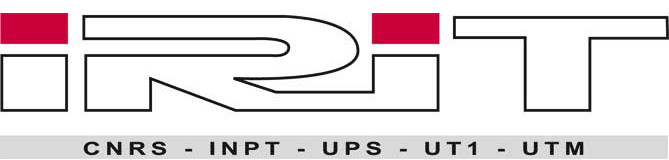
\includegraphics[width=0.28\textwidth]{logos/logo-irit.jpg}}
	\fancyhead[C]{} % On enlève les informations du header
	\fancyfoot[C]{} % On enlève les informations du footer
	\renewcommand{\headrulewidth}{0pt} % On enlève la ligne du header
} \Huge
\fancypagestyle{body}{%
	\restoregeometry 
	\pagestyle{fancy}
	\fancyhf{}
	\fancyhead[LO]{\ifthenelse{\equal{\value{chapter}}{0}}{}{\thesection. \rightmark}} %rightmark = section
	\fancyhead[RE]{\ifthenelse{\equal{\value{chapter}}{0}}
		{}
		{Chapter \thechapter.}
		\leftmark
	} %leftmark = chapter
	\fancyhead[RO]{\thepage} %
	\fancyhead[LE]{\thepage} %
	\renewcommand*{\chaptermark}[1]{\markboth{##1}{}}
	\renewcommand*{\sectionmark}[1]{\markright{##1}{}}
	\renewcommand\headrulewidth{.1pt}
%	\setlength{\parskip}{0.3cm} % Espace entre paragraphes
%	\renewcommand{\arraystretch}{1.5} % Espace entre cases d'un tableau
}
\fancypagestyle{plain}{
	\pagestyle{body}
	\fancyhead[LO]{\rightmark}
}
\fancypagestyle{appendix}{%
	\restoregeometry
	% On nettoie les headers et footers existants de "fancy"
	\fancyhf{}
	% Pour le header
	\fancyhead[RE]{Appendix}
	\fancyhead[LO]{\thechapter. \leftmark} %leftmark = chapter
	\fancyhead[RO]{\thepage} %
	\fancyhead[LE]{\thepage} %
	\renewcommand*{\chaptermark}[1]{\markboth{##1}{}}
	\renewcommand\headrulewidth{.1pt}
	% Pour le footer
	%\fancyfoot[C]{\thepage}
	\renewcommand\footrulewidth{0pt}
}
% \newacronymwithdescr{Label}{Court}{Long}{Description}
\newcommand*{\newacronymwithdescr}[5][]{%
  \newglossaryentry{main-#2}{name={#3},%
  text={(\acs{#2}) #3\glsadd{#2}},%
  description={#5},%
  #1
  }%
  \newacronym{#2}{#3\glsadd{main-#2}}{#4}%
}

% Pas de point final pour les entrées glossaire ou acronymes
\setacronymstyle{sm-short-long}
%\newacronym{IMT}{IMT}{Institut de Mathématiques de Toulouse}
\newacronymwithdescr{IMT}{IMT}{Institut de Mathématiques de Toulouse}{is the main laboratory in mathematics in Toulouse}
\newglossaryentry{Blabla}{name=Blabla,description={is....}}

% To use the glossary entries:
% \acs{} (for short one)
% \ac{} (for long one - only on first appearence)


% MACROS

% Couleurs pour les corrections
\newcommand {\JY}[1] {\textcolor{red}{#1}}
\newcommand {\FR}[1] {\textcolor[rgb]{0.0,0.3,0.0}{#1}}
\newcommand {\OL}[1] {\textcolor{blue}{#1}}
\newcommand {\HW}[1] {\textcolor[rgb]{0.3,0.2,0.0}{#1}}
%\newcommand{\hilite}[1] {\emph{#1}}
\newcommand{\hilite}[1] {\Req{#1}}
\newcommand {\Req}[1] {\textcolor[rgb]{0.75,0.0,0.0}{#1}}
\newcommand {\Geq}[1] {\textcolor[rgb]{0.0,0.5,0.0}{#1}}
\newcommand {\Beq}[1] {\textcolor[rgb]{0.0,0.15,0.60}{#1}}
\newcommand {\black}[1] {\textcolor{black}{#1}}

% Espaces mathématiques
\newcommand {\DPUN} {{\mathcal D}}
\newcommand {\DTREE} {{\mathcal D}^e}
\newcommand {\CC} {\mathbb C}
\newcommand {\RR} {\mathbb R}
\newcommand {\RP} {\mathbb R^{\mathcal P}}
\newcommand {\RPE} {\mathbb R^{\mathcal P \times |\edges |}}
\newcommand {\codeset} {\mathbb R^{\mathcal P \times \leaves}}
\newcommand {\Dset} {\mathbb R^{\mathcal P \times (\mathcal P \#\leaves) }}
\newcommand {\ZZ} {\mathbb Z}
\newcommand {\NN} {\mathbb N}
\newcommand {\PP} {{\mathcal P}}
\newcommand {\HH} {{\mathbb H}}
\newcommand {\II} {{\mathbb I}}
\renewcommand {\SS} {{\mathcal S}} % applis supports
\newcommand {\SA} {{\mathbb S}} % support accessible

% Fonctions
\newcommand {\f}[1] { {\mathcal F}\left( #1 \right) }
\newcommand {\F}[1] { {\mathcal F^{-1}}\left( #1 \right) }
\newcommand {\norm}[2] {\left\| #1 \right\| _{#2}}
\newcommand {\defeq} {\triangleq}

% Opérateurs
\DeclareMathOperator {\sign} {sign}
\DeclareMathOperator {\prox} {prox}
\DeclareMathOperator {\argmin} {argmin}
\DeclareMathOperator {\supp} {supp}
\DeclareMathOperator {\rg} {rg}
\DeclareMathOperator {\diag} {diag}
\newcommand {\RG}[1] {\rg\left( #1 \right)}
\newcommand {\SUPP}[1] {\supp\left( #1 \right)}
\newcommand {\PS}[2] {\langle #1 , #2 \rangle}
\newcommand {\PROBA}[1] {\mathbb P \left( #1 \right)}
\newcommand {\one}[1] {\mathbbm{1}_{ #1 }}
%\newcommand {\one}[1] {\chi_{ #1 }} %{\mathbbm{1}_{ #1 }}
\newcommand {\oneinf}[1] {\chi_{ #1 }}
%\newcommand {\oneinf}[1] {{\mathcal I}_{ #1 }} 

% Acronymes
\newcommand {\PSNR} { \textrm{PSNR}^* } 
\newcommand {\NRE} { \textrm{NRE} }
\newcommand {\CPR} { \textrm{RER} }
\newcommand {\COST} { \textrm{G} } % ancien compression ratio

% Raccourcis
\newtheorem{prop}{Proposition}[section]

\newcommand {\nodes} {\mathcal N}
\newcommand {\edges} {\mathcal E}
\newcommand {\leaves} {\mathcal L}
\newcommand {\NL} {\#\leaves}
\newcommand {\hall} {h^e _{e \in \edges}}
%\newcommand {\multiconv}[1] { \bigstar_{\substack{#1}}\, }
\newcommand {\multiconv}[1] { \mathbf h^{#1}\, }
\newcommand {\tpath}[1] {\mathcal{C}(#1)}
\newcommand {\code} {\mathbf x}
\newcommand {\data} {\mathbf y}
\newcommand {\dataex} {\mathbf b}
\newcommand {\databis} {\mathbf y^e}
\newcommand {\D} {\mathbf D}
\newcommand {\Hs} {\mathbf A}
\newcommand {\Ha} {\mathbf H}
\newcommand {\Haf} {\hat{\mathbf H}}
\newcommand {\Hab} {\bar{\mathbf H}}
\newcommand {\res} {\mathbf r}

\newcommand {\tree}{\mathcal T}
\newcommand{\subtree}[1]{\tree^{#1}}

\newcommand {\stopalgo}{\epsilon}

% autres MACROS
\newcommand {\hkall} {(h^k)_{1 \leq k \leq K}}
\newcommand {\hkconv} {h^1 * \dots * h^K}
\newcommand {\hkconvnorm} {\frac{h^1}{\norm{h^1}{2}} * \dots * \frac{h^K}{\norm{h^K}{2}}}
\newcommand {\hkconvp} {g^{1} * \dots * g{K}}
\newcommand {\hkconvs} {f^{1} * \dots * f^{K}}
\newcommand {\fobj} {\| \code * h^1 * \dots * h^K - \data \|_2^2}
\newcommand {\fobjlambda} {\| \lambda \code * h^1 * \dots * h^K - \data \|_2^2}

% Macros added by Mael
\newcommand{\file}{\texttt}
\newcommand{\dispCode}{\texttt}
\newcommand{\dispCodeLong}[1]{
\begin{verbatim} #1 \end{verbatim}
}
\DeclareMathOperator*{\argmax}{\arg\!\max}% http://tex.stackexchange.com/q/83169/5764

\algnewcommand\algorithmicinput{\textbf{Input:}}
\algnewcommand\Input{\item[\algorithmicinput]}
\algnewcommand\algorithmicoutput{\textbf{Output:}}
\algnewcommand\Output{\item[\algorithmicoutput]}

 % <-- all the \usepackages
\fancypagestyle{titlepage}{% 
	\lhead{
\includegraphics[width=0.30\textwidth]{logos/logo-enseeiht.png}}
	\rhead{
\includegraphics[width=0.30\textwidth]{logos/logo-imt.jpg}}
	\lfoot{
\includegraphics[width=0.28\textwidth]{logos/logo-univ-ups.png}}
	\rfoot{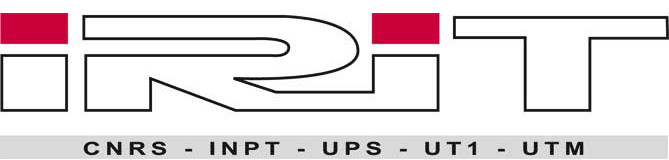
\includegraphics[width=0.28\textwidth]{logos/logo-irit.jpg}}
	\fancyhead[C]{} % On enlève les informations du header
	\fancyfoot[C]{} % On enlève les informations du footer
	\renewcommand{\headrulewidth}{0pt} % On enlève la ligne du header
} \Huge
\fancypagestyle{body}{%
	\restoregeometry 
	\pagestyle{fancy}
	\fancyhf{}
	\fancyhead[LO]{\ifthenelse{\equal{\value{chapter}}{0}}{}{\thesection. \rightmark}} %rightmark = section
	\fancyhead[RE]{\ifthenelse{\equal{\value{chapter}}{0}}
		{}
		{Chapter \thechapter.}
		\leftmark
	} %leftmark = chapter
	\fancyhead[RO]{\thepage} %
	\fancyhead[LE]{\thepage} %
	\renewcommand*{\chaptermark}[1]{\markboth{##1}{}}
	\renewcommand*{\sectionmark}[1]{\markright{##1}{}}
	\renewcommand\headrulewidth{.1pt}
%	\setlength{\parskip}{0.3cm} % Espace entre paragraphes
%	\renewcommand{\arraystretch}{1.5} % Espace entre cases d'un tableau
}
\fancypagestyle{plain}{
	\pagestyle{body}
	\fancyhead[LO]{\rightmark}
}
\fancypagestyle{appendix}{%
	\restoregeometry
	% On nettoie les headers et footers existants de "fancy"
	\fancyhf{}
	% Pour le header
	\fancyhead[RE]{Appendix}
	\fancyhead[LO]{\thechapter. \leftmark} %leftmark = chapter
	\fancyhead[RO]{\thepage} %
	\fancyhead[LE]{\thepage} %
	\renewcommand*{\chaptermark}[1]{\markboth{##1}{}}
	\renewcommand\headrulewidth{.1pt}
	% Pour le footer
	%\fancyfoot[C]{\thepage}
	\renewcommand\footrulewidth{0pt}
}
% \newacronymwithdescr{Label}{Court}{Long}{Description}
\newcommand*{\newacronymwithdescr}[5][]{%
  \newglossaryentry{main-#2}{name={#3},%
  text={(\acs{#2}) #3\glsadd{#2}},%
  description={#5},%
  #1
  }%
  \newacronym{#2}{#3\glsadd{main-#2}}{#4}%
}

% Pas de point final pour les entrées glossaire ou acronymes
\setacronymstyle{sm-short-long}
%\newacronym{IMT}{IMT}{Institut de Mathématiques de Toulouse}
\newacronymwithdescr{IMT}{IMT}{Institut de Mathématiques de Toulouse}{is the main laboratory in mathematics in Toulouse}
\newglossaryentry{Blabla}{name=Blabla,description={is....}}

% To use the glossary entries:
% \acs{} (for short one)
% \ac{} (for long one - only on first appearence)


% MACROS

% Couleurs pour les corrections
\newcommand {\JY}[1] {\textcolor{red}{#1}}
\newcommand {\FR}[1] {\textcolor[rgb]{0.0,0.3,0.0}{#1}}
\newcommand {\OL}[1] {\textcolor{blue}{#1}}
\newcommand {\HW}[1] {\textcolor[rgb]{0.3,0.2,0.0}{#1}}
%\newcommand{\hilite}[1] {\emph{#1}}
\newcommand{\hilite}[1] {\Req{#1}}
\newcommand {\Req}[1] {\textcolor[rgb]{0.75,0.0,0.0}{#1}}
\newcommand {\Geq}[1] {\textcolor[rgb]{0.0,0.5,0.0}{#1}}
\newcommand {\Beq}[1] {\textcolor[rgb]{0.0,0.15,0.60}{#1}}
\newcommand {\black}[1] {\textcolor{black}{#1}}

% Espaces mathématiques
\newcommand {\DPUN} {{\mathcal D}}
\newcommand {\DTREE} {{\mathcal D}^e}
\newcommand {\CC} {\mathbb C}
\newcommand {\RR} {\mathbb R}
\newcommand {\RP} {\mathbb R^{\mathcal P}}
\newcommand {\RPE} {\mathbb R^{\mathcal P \times |\edges |}}
\newcommand {\codeset} {\mathbb R^{\mathcal P \times \leaves}}
\newcommand {\Dset} {\mathbb R^{\mathcal P \times (\mathcal P \#\leaves) }}
\newcommand {\ZZ} {\mathbb Z}
\newcommand {\NN} {\mathbb N}
\newcommand {\PP} {{\mathcal P}}
\newcommand {\HH} {{\mathbb H}}
\newcommand {\II} {{\mathbb I}}
\renewcommand {\SS} {{\mathcal S}} % applis supports
\newcommand {\SA} {{\mathbb S}} % support accessible

% Fonctions
\newcommand {\f}[1] { {\mathcal F}\left( #1 \right) }
\newcommand {\F}[1] { {\mathcal F^{-1}}\left( #1 \right) }
\newcommand {\norm}[2] {\left\| #1 \right\| _{#2}}
\newcommand {\defeq} {\triangleq}

% Opérateurs
\DeclareMathOperator {\sign} {sign}
\DeclareMathOperator {\prox} {prox}
\DeclareMathOperator {\argmin} {argmin}
\DeclareMathOperator {\supp} {supp}
\DeclareMathOperator {\rg} {rg}
\DeclareMathOperator {\diag} {diag}
\newcommand {\RG}[1] {\rg\left( #1 \right)}
\newcommand {\SUPP}[1] {\supp\left( #1 \right)}
\newcommand {\PS}[2] {\langle #1 , #2 \rangle}
\newcommand {\PROBA}[1] {\mathbb P \left( #1 \right)}
\newcommand {\one}[1] {\mathbbm{1}_{ #1 }}
%\newcommand {\one}[1] {\chi_{ #1 }} %{\mathbbm{1}_{ #1 }}
\newcommand {\oneinf}[1] {\chi_{ #1 }}
%\newcommand {\oneinf}[1] {{\mathcal I}_{ #1 }} 

% Acronymes
\newcommand {\PSNR} { \textrm{PSNR}^* } 
\newcommand {\NRE} { \textrm{NRE} }
\newcommand {\CPR} { \textrm{RER} }
\newcommand {\COST} { \textrm{G} } % ancien compression ratio

% Raccourcis
\newtheorem{prop}{Proposition}[section]

\newcommand {\nodes} {\mathcal N}
\newcommand {\edges} {\mathcal E}
\newcommand {\leaves} {\mathcal L}
\newcommand {\NL} {\#\leaves}
\newcommand {\hall} {h^e _{e \in \edges}}
%\newcommand {\multiconv}[1] { \bigstar_{\substack{#1}}\, }
\newcommand {\multiconv}[1] { \mathbf h^{#1}\, }
\newcommand {\tpath}[1] {\mathcal{C}(#1)}
\newcommand {\code} {\mathbf x}
\newcommand {\data} {\mathbf y}
\newcommand {\dataex} {\mathbf b}
\newcommand {\databis} {\mathbf y^e}
\newcommand {\D} {\mathbf D}
\newcommand {\Hs} {\mathbf A}
\newcommand {\Ha} {\mathbf H}
\newcommand {\Haf} {\hat{\mathbf H}}
\newcommand {\Hab} {\bar{\mathbf H}}
\newcommand {\res} {\mathbf r}

\newcommand {\tree}{\mathcal T}
\newcommand{\subtree}[1]{\tree^{#1}}

\newcommand {\stopalgo}{\epsilon}

% autres MACROS
\newcommand {\hkall} {(h^k)_{1 \leq k \leq K}}
\newcommand {\hkconv} {h^1 * \dots * h^K}
\newcommand {\hkconvnorm} {\frac{h^1}{\norm{h^1}{2}} * \dots * \frac{h^K}{\norm{h^K}{2}}}
\newcommand {\hkconvp} {g^{1} * \dots * g{K}}
\newcommand {\hkconvs} {f^{1} * \dots * f^{K}}
\newcommand {\fobj} {\| \code * h^1 * \dots * h^K - \data \|_2^2}
\newcommand {\fobjlambda} {\| \lambda \code * h^1 * \dots * h^K - \data \|_2^2}

% Macros added by Mael
\newcommand{\file}{\texttt}
\newcommand{\dispCode}{\texttt}
\newcommand{\dispCodeLong}[1]{
\begin{verbatim} #1 \end{verbatim}
}
\DeclareMathOperator*{\argmax}{\arg\!\max}% http://tex.stackexchange.com/q/83169/5764

\algnewcommand\algorithmicinput{\textbf{Input:}}
\algnewcommand\Input{\item[\algorithmicinput]}
\algnewcommand\algorithmicoutput{\textbf{Output:}}
\algnewcommand\Output{\item[\algorithmicoutput]}
\author{Maël Valais}
\date{Updated on \today}
\title{Optimization of dictionaries structured in convolutional trees for sparse image representation - Master's Thesis}
\begin{document}
\begin{titlepage}
\thispagestyle{pagedegarde}
\newgeometry{tmargin=2.2cm,bmargin=4cm,lmargin=2cm,rmargin=2cm}
\begin{center}
\topskip2.8cm
\textsc{Université Toulouse III — Paul Sabatier}\\
\vspace{0.5 cm}
\line(1,0){100}\\
\vspace{0.6 cm}
{{{Internship Report}}}\\
\vspace{0.3cm}
Defended on September 15\th, 2016\\ \vspace{0.3 cm} par\\ \vspace{0.3 cm} \textbf{Maël \textsc{Valais}}\\
\vfill
{\Huge \textbf{Optimization of dictionaries structured as convolutions trees for sparse image representation }}\\
\vfill

{{Internship at \acs{IMT}}}\\
{Université Paul Sabatier}\\
{118, route de Narbonne}\\
{31400 Toulouse}\\
\vspace{2 cm}

\par Supervised by \\ \textbf{François \textsc{Malgouyres}}\\
Institut de Mathématiques de Toulouse\\ 
%\vspace{1cm}
\par and \\Jean-Yves \textbf{ \textsc{Tourneret}}\\
ENSEIHHT, Toulouse
\end{center}
\end{titlepage}

% Préparation pour les pages de corps
\pagestyle{empty}
\restoregeometry
\cleardoublepage % Blanc jusqu'à prochaîne page paire

\tableofcontents
{\let\clearpage\relax\listoffigures}
{\let\clearpage\relax\listoftables}
{\let\clearpage\relax\listofalgorithms}

\pagestyle{corps} % Uncomment to show title page

\chapter{Introduction}

\section{The need for sparse representations}

A sparse signal over some representation means that it can be written with as few information as possible – in other words, sparse means with many zeros. Many applications spanning from machine learning to image denoising heavily rely on the property that we can summarize – or more precisely approximate – any signal using a proper representation. The job of obtaining the raw\footnote{Any raw signal is actually represented by the canonical basis} signal from its sparse counterpart takes the form of an operator, often called dictionary or transform.

This chapter will review the main existing dictionaries in use for sparse representation, spanning from non-adaptative transforms to learned dictionaries and going through the intermediate over-complete dictionaries.

\section{Non-adaptative dictionaries}

The Fourier transform is a classical example of operators used for sparsity. In figure \ref{fig_fourier}, the left picture $\y$ has been represented using a Fourier basis, which can be written as a matrix $\D$. The right picture shows the coefficients $\x$ such that
$$\D^T\y = \x$$


\begin{figure}[!ht]
\subcaptionbox{Picture $\y$ with many discontinuities.}%
  [.49\linewidth]{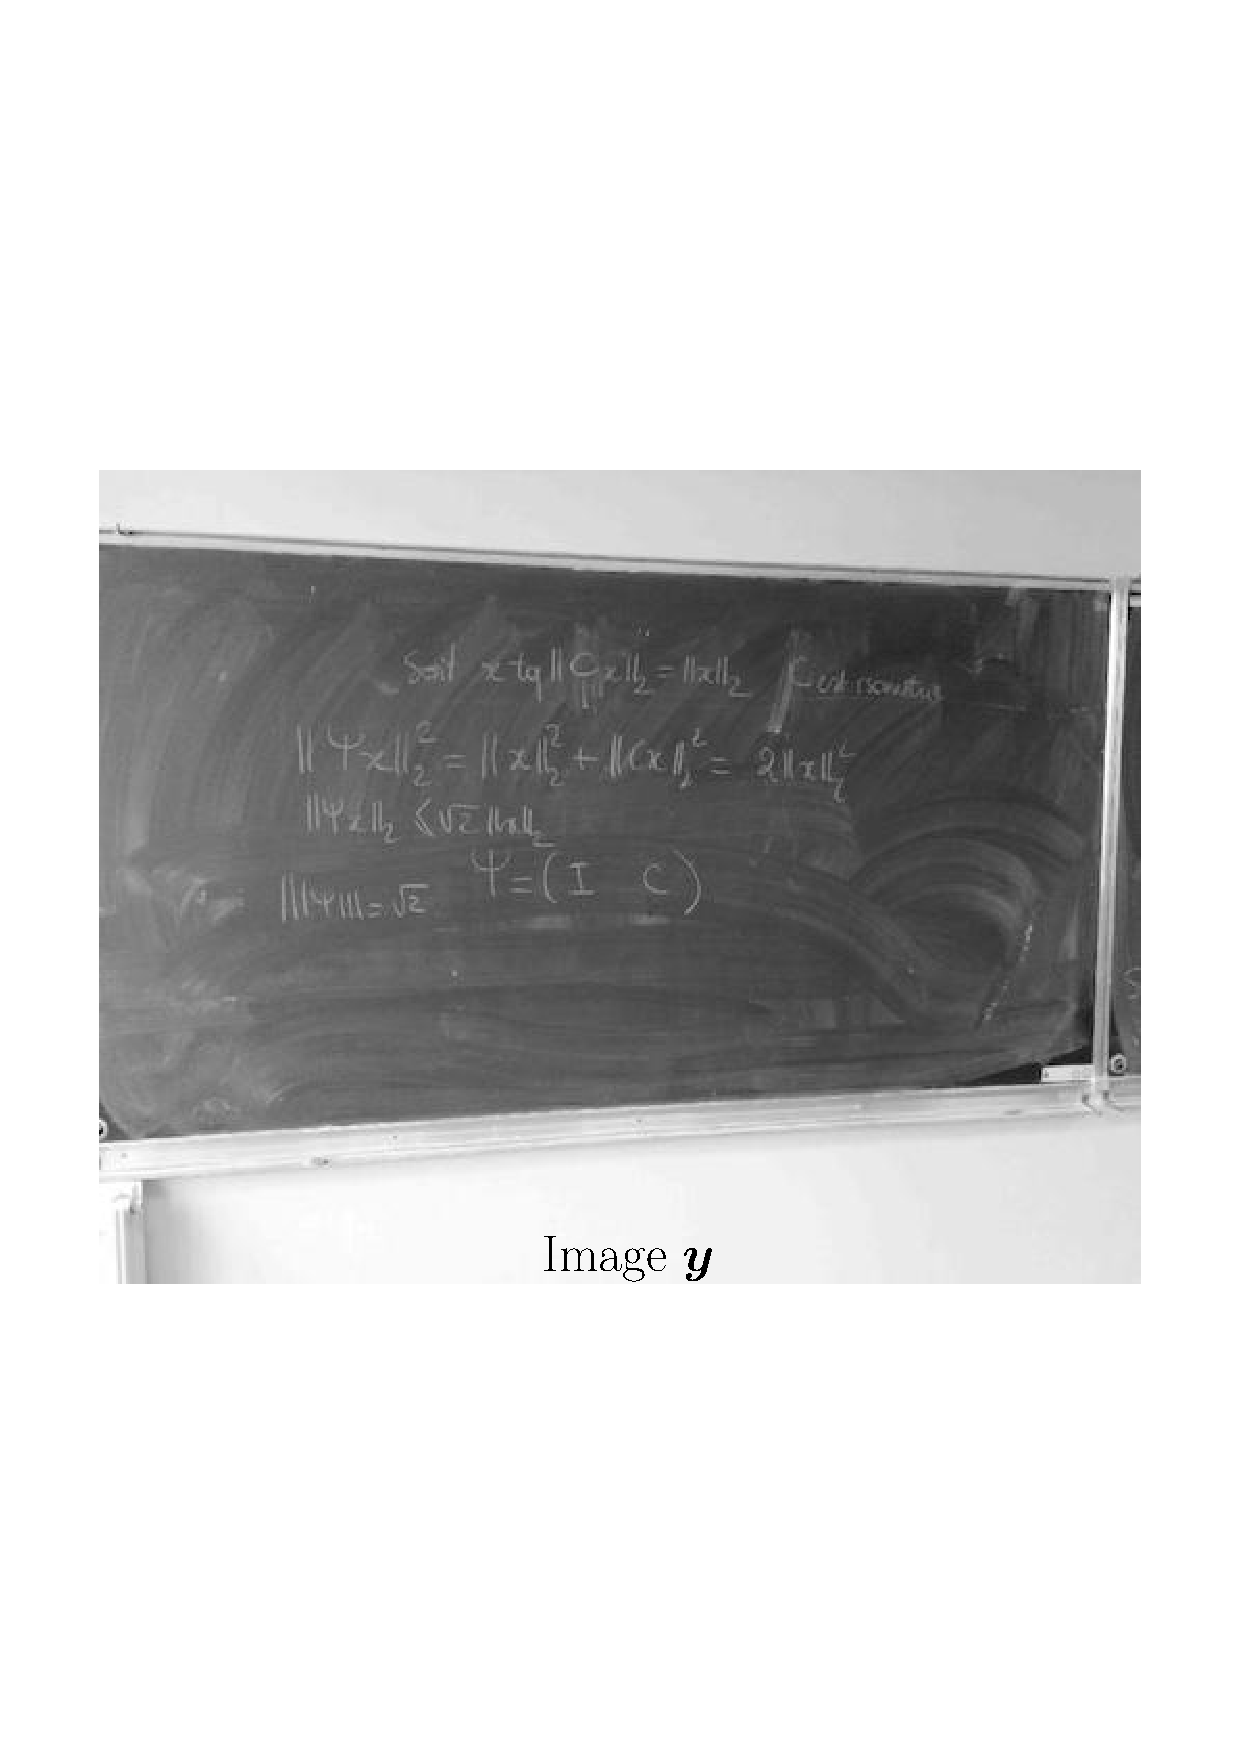
\includegraphics[width=0.49\textwidth]{figures/exple_fourier_spacial.pdf}}
 \subcaptionbox{Result of applying the Fourier transform to $\y$}%
  [.49\linewidth]{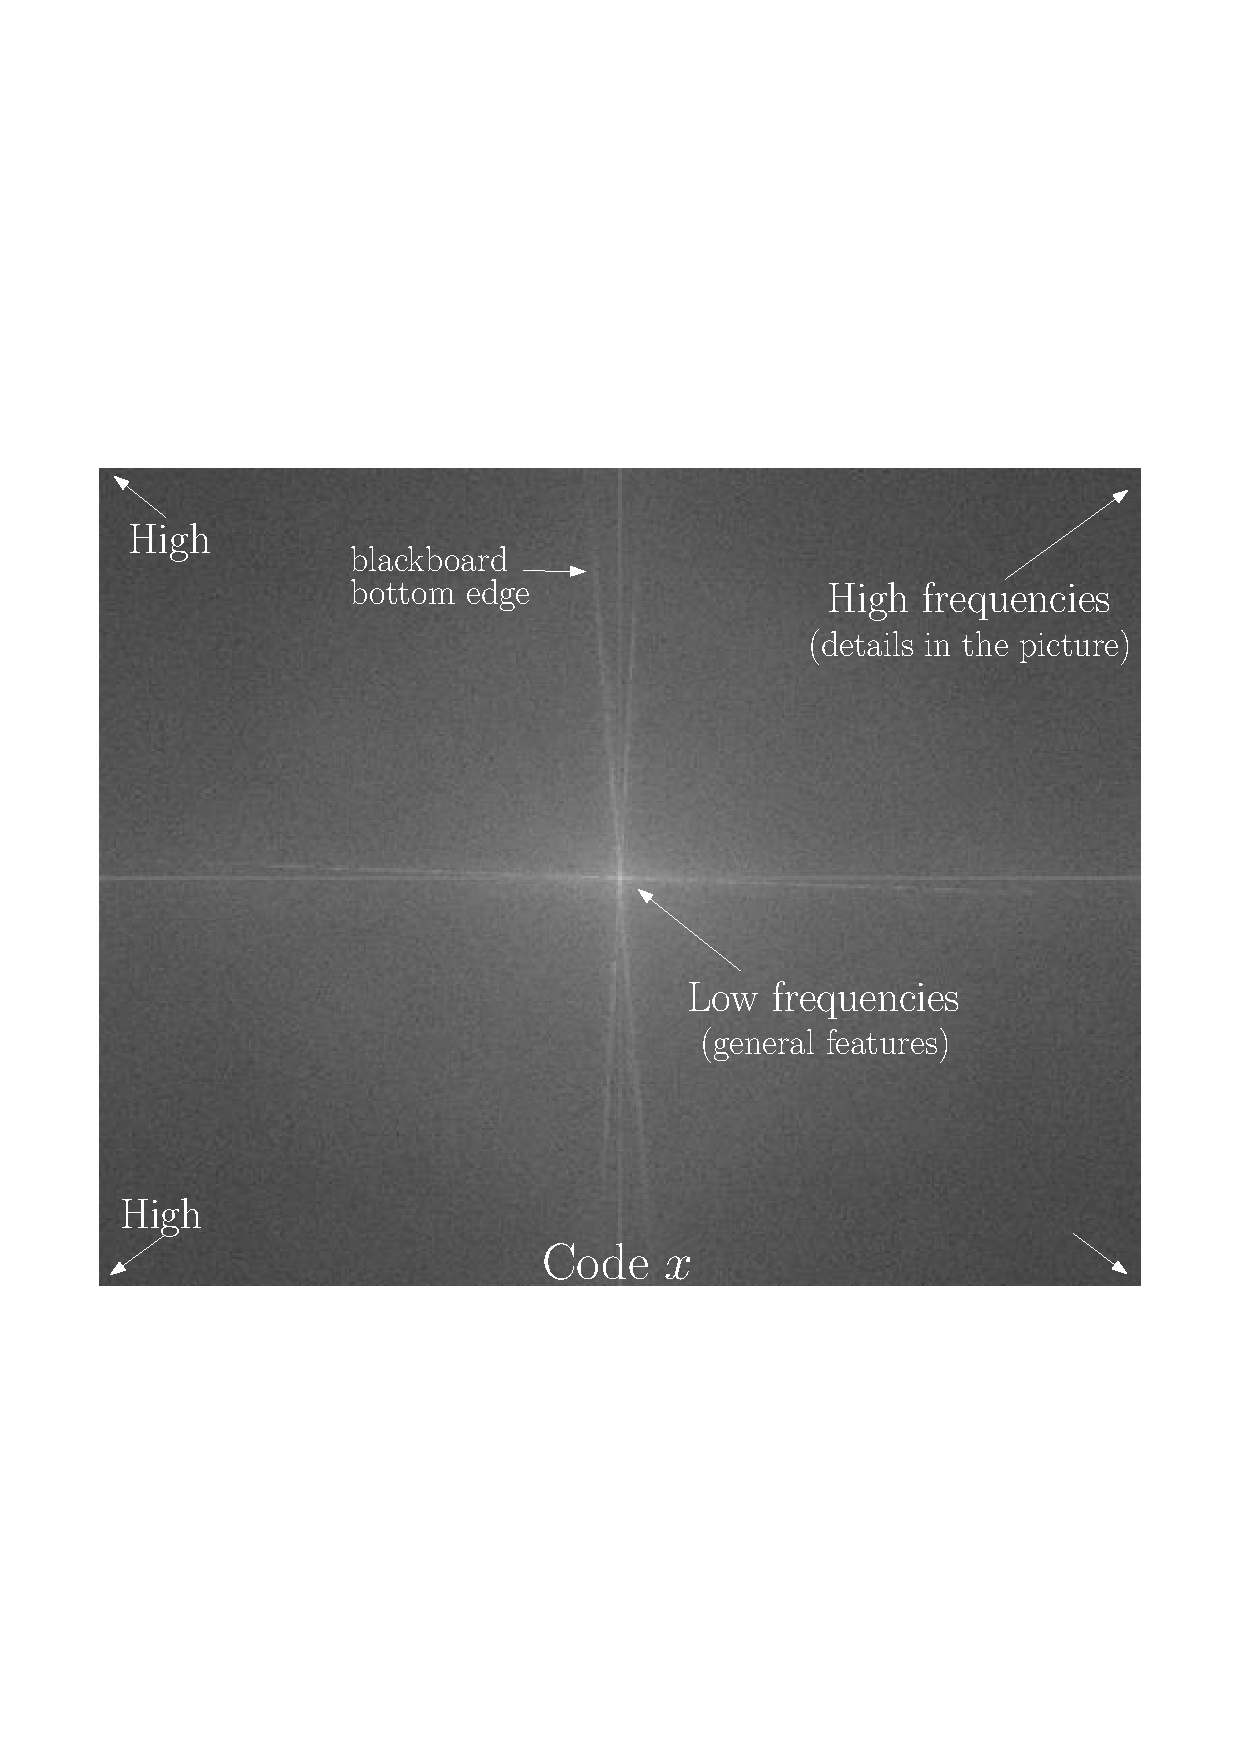
\includegraphics[width=0.49\textwidth]{figures/exple_fourier_frequen.pdf}}
  \caption{Decomposition $\D^T\y=\x$ of a signal $\y$ using the dictionary $\D$ made of Fourier series. In $\x$, the middle coefficients are coding for "large" features while the corner values are coding for the details. The multiple white lines, spanning from the middle to the borders, outline the discontinuities caused by the edges of the blackboard; the coefficients are scattered (not sparse), which shows that Fourier has trouble when dealing with discontinuities.} \label{fig_fourier}
\end{figure}

But the Fourier transform is quite different from the representations we have in mind, namely the convolutional tree structure. First, it is a linear mapping and its associated matrix forms a basis. This representation one-to-one in the sense that every code $\x$ has a unique image $\y$. Also, Fourier's basis is orthogonal, meaning that the operator is stable (it does not amplify errors). % TODO Finally, the basis is normed, meaning that...

More importantly, Fourier has interesting properties that allow fast implementations. For example, applying the Matlab function \texttt{fft2} on the \cref{fig_fourier} is extremely fast. Instead of computing an time-expensive $O(N^2)$\footnote{$N$ is the dimension of the concatenated image, if we consider the image as a vector} matrix-vector product, the fast Fourier transform only require a $O(NlogN)$ time.

The Fourier transform is widely used as an operator for sparse representations, mainly when dealing with smooth signals that can be approximated by a sum of sines. But this operator does not do well on images: they contain many discontinuities and are far from being representable using sines. Most of the coefficients of code $\x$ in \cref{fig_fourier} are non-zero. But something worse happens on the edges of the blackboard: the white vertical and horizontal lines that are full of high-value coefficients are trying to code for the discontinuity, which is quite far from possible in Fourier basis.

Along with Fourier, many other non-adaptative dictionaries exist; we can mention the cosine transform which is at the core of JPEG compression. We can also cite the wavelet transform, used in JPEG2000 compression (for movies in theaters), and the curvelet transform, which is more tolerant to non-smooth images. And as for Fourier, wavelet and curvelet transforms both have fast implementations.


\section{Adaptative dictionaries}
Right before the first learned dictionaries, \cite{chen_atomic_2001} extended the basis-based dictionaries using multiple basis to form an over-complete dictionary. Doing so would increase the expressivity of such representations, although making the inverse transform less obvious. % TODO overcomplete implies what?

Learned dictionaries take the same bet of over-completeness. But instead of choosing multiple fixed basis, we optimize the dictionary matrix so that the atoms (other name for the columns of the dictionary matrix) generate the sparsest representations for a given set of images.

The \cref{fig_overcomplete_matrix} shows the matrix-vector product of a sparse code $\x$ and a learned $\D$, giving an approximation of $\y$. For this example, $\y$ will be represented by a linear combination of three atoms of $\D$.


\begin{figure}[!ht] \centering
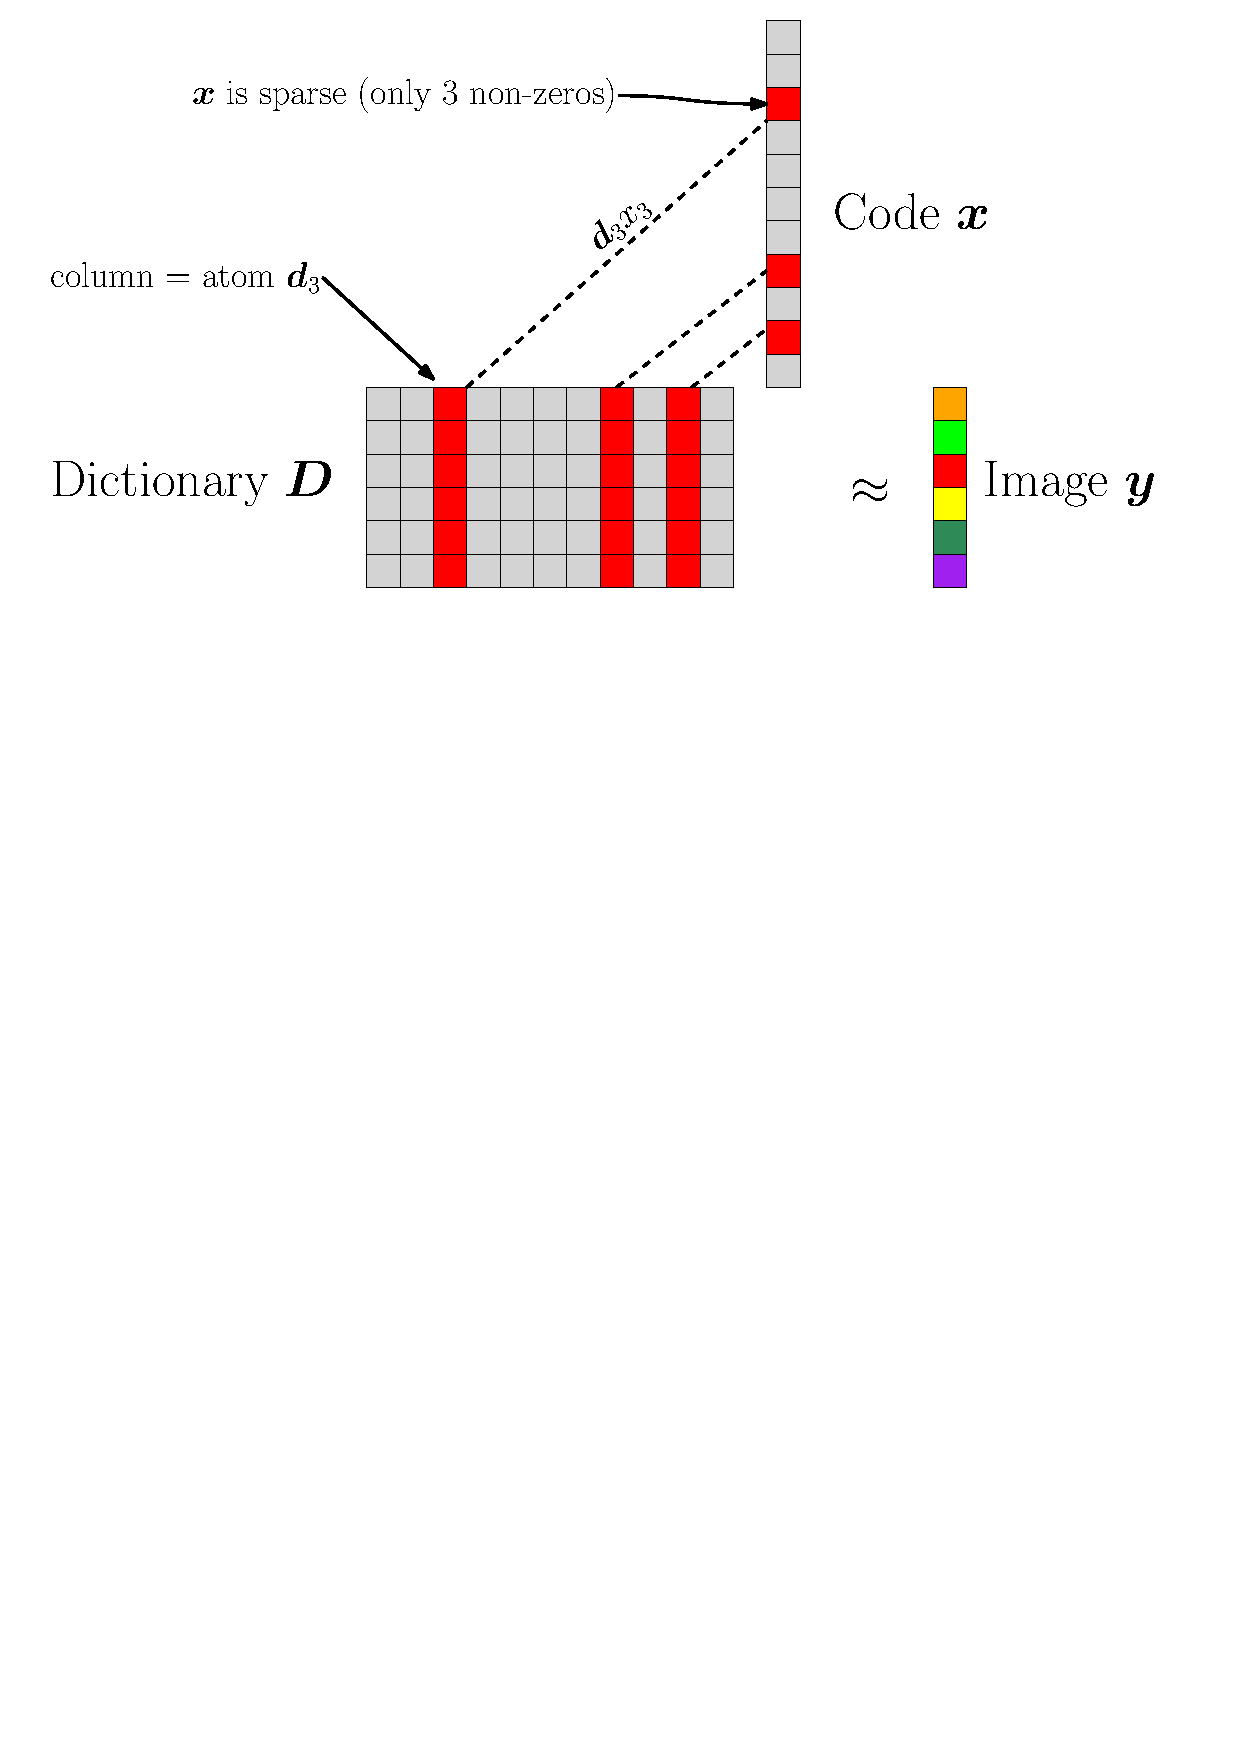
\includegraphics[width=0.45\textwidth]{figures/sparsity-matrix.pdf}
\caption{Matrix view of $\D\x$ when $\D$ is over-complete (much more columns than lines). $\y$ can be represented using a few atoms of $\D$.} \label{fig_overcomplete_matrix}
\end{figure}


Given a set of sample images $\displaystyle \Y = \begin{bmatrix} \y_1 & \dots & \y_S \end{bmatrix}$ (images are "flattened" into vectors $\y_i$ of size $N$), the dictionary learning optimization problem is defined as

\begin{align}\label{eq_dict_learn}
	 (DL) && \underset{\D,\X}{\min}~ \lambda \lVert \x \rVert_1 + \lVert \D\X - \Y \rVert^2_2
\end{align} 

% TODO WARNING! ||X||_1 doesn't exist, ||Y||_2 either
with $\lVert . \rVert_2$ denoting the euclidian norm, $\lVert . \rVert_1$ the $l_1$ norm defined by $\lVert \x \rVert_1 = \sum_{i,j} |\x_i|$, $\X = \begin{bmatrix} \x_1 & \dots & \x_s \end{bmatrix}$ the matrix containing the sparse representations $\x_i$ of size $K$ for all images in $\Y$ and $\D \in \mathcal{M}^{K \times N}$ the dictionary.

\section{K-SVD algorithm}

\ac{KSVD}, first introduced in \cite{aharon_k-svd:_2006}, is a well known algorithm for dictionary learning (except that it does not actually solve the above problem \cref{eq_dict_learn}). As many of the concepts behind the PALMTREE algorithm developed in \cite{chabiron_optimization_2016} come from the K-SVD algorithm, this section will introduce it. % TODO Why KSVD != dict. learning problem 

Here is the problem that K-SVD is solving, which is a "stronger" version of (DL) in the sense that the level of sparsity in K-SVD is enforced:
\begin{equation*}  \begin{aligned}
(DL_{\text{strong}}) && \underset{\D,\X}{\min}~ & \lVert \D\X-\Y \rVert^2_F \\
&& s.t.~& \lVert \x_i \rVert_0 \le \gamma & \quad \forall i \text{ in } 1..S
\end{aligned} \label{eq_ksvd} \end{equation*}

with $F$ the Frobenius norm and $\x_i$ the i-th column of $\X$.

\ac{KSVD} learns the dictionary by alternatively optimizing $\x$ and $\D$. Optimizing $\x$ is the sparse coding phase, and optimizing $\D$ is the dictionary update phase.

\begin{algorithm}
    \caption{K-SVD (K-Singular Value Decomposition) algorithm for (DL)}
  \begin{algorithmic}[0]
    \Input signal samples $(\y_i)_{i=1..N}$ forming columns of $\Y \in \mathbb{R}^{S \times N}$
    \Output dictionary $\D \in \mathbb{R}^{K \times N}$ with $K>>N$
    \State \textbf{Initialization} Initialize $\D$ s.t.~every column is $l^2$ normalized
    \While{convergence}
	\State For each image $i$, solve \Comment{Sparse coding step}
		\begin{align}
			\quad \min_{\x_i}~ & \lVert \y_i-\D\x_i\rVert^2\\
			s.t.~& \lVert \x_i \rVert_0 \le \gamma \notag
		\end{align}
	\State Set $\D^{old} \leftarrow \D$
	\State For each atom $k$ of $\D^{old}$, \Comment{Dictionary update step}
	\begin{enumerate}[leftmargin=15mm,label=(\alph*)]
		\item find the images $\y_i$ that use the atom $\d_k$, meaning $\x_i^k \ne 0$ \label{item_atom_used}
		\item compute the error matrix associated to this atom,
		\begin{align}
			E_k =& Y-\sum_{i\ne k} {d_i}^T\x_i
		\end{align}
		\item keep only columns of $\bm{E}_k$ found in \ref{item_atom_used}
		\item Apply SVD decomposition $\bm{E}_k - \bm{U} \Delta V^T$. The first column of $\bm{U}$ becomes the new $\d_k$. $\x_k$ is updated using the first column of $\bm{V}$ multiplied by $\Delta(1,1)$ (highest Eigen value)
	\end{enumerate}
    \EndWhile
  \end{algorithmic}
\end{algorithm}
\section{The seek for fast transforms}

... talk about the problem of need for small patches and resolution limits in KSVD % TODO KSVD problems

As K-SVD relies on the $O(NK)$ matrix-vector product and that a dictionary achieves sparsity as long as $K >> N$, we easily understand that $N$ cannot be big. When implemented, K-SVD atoms (called patches because of their size) are at most $16 \times 16$.

Also, the K-SVD is translation-sensitive in the sense that multiple atoms of the dictionary are only different by translation. In PALMTREE, the "final" convolutions between the atoms $h^{*l}$ and $\x^l$ adresses this issue.

% TODO add KSVD image
% TODO Malgouyres: talk about other models (???)

\section{PALMTREE algorithm}

\subsection{Dictionary-as-a-tree model \label{sec_tree_model}}
The current work, developed in \cite{chabiron_toward_2015} and \cite{chabiron_optimization_2016} propose a different way of structuring the matrix $\D$. Instead of using "plain" atoms as columns and dealing with the matrix-vector product in $O(N^2)$, $\D$ is defined by a tree structure $\T(\V,\E)$. 

The root $r$ and leaves $l$ vertex in $\V$ allow to define a branch as the successive edges growing from the root to one of the leaves.

Every edge $e$ in $\E$ bears a kernel $\h^e$ and a support $\s^e$. If the target image $\y$ has its pixels in a "flattened" one-dimensional space $\P$, with
$$\y : \P \rightarrow \mathbb{R}$$
then every kernel $\h^e$ and support $\s^e$ are also defined on $\P$ by 
$$\h^e:\P \rightarrow \mathbb{R}$$ 
$$\s^e:\P \rightarrow \{0,1\}$$

The figure \ref{fig_example_kernel} exhibits an example of standard kernel filter on the left, and a $\h^e$kernel on the right. The numerical values are the values of $\h^e$ while the gray squares are the locations where $\h^e$ has the right to have values on (i.e. the support $\s^e$).

\begin{figure}[!ht]\centering
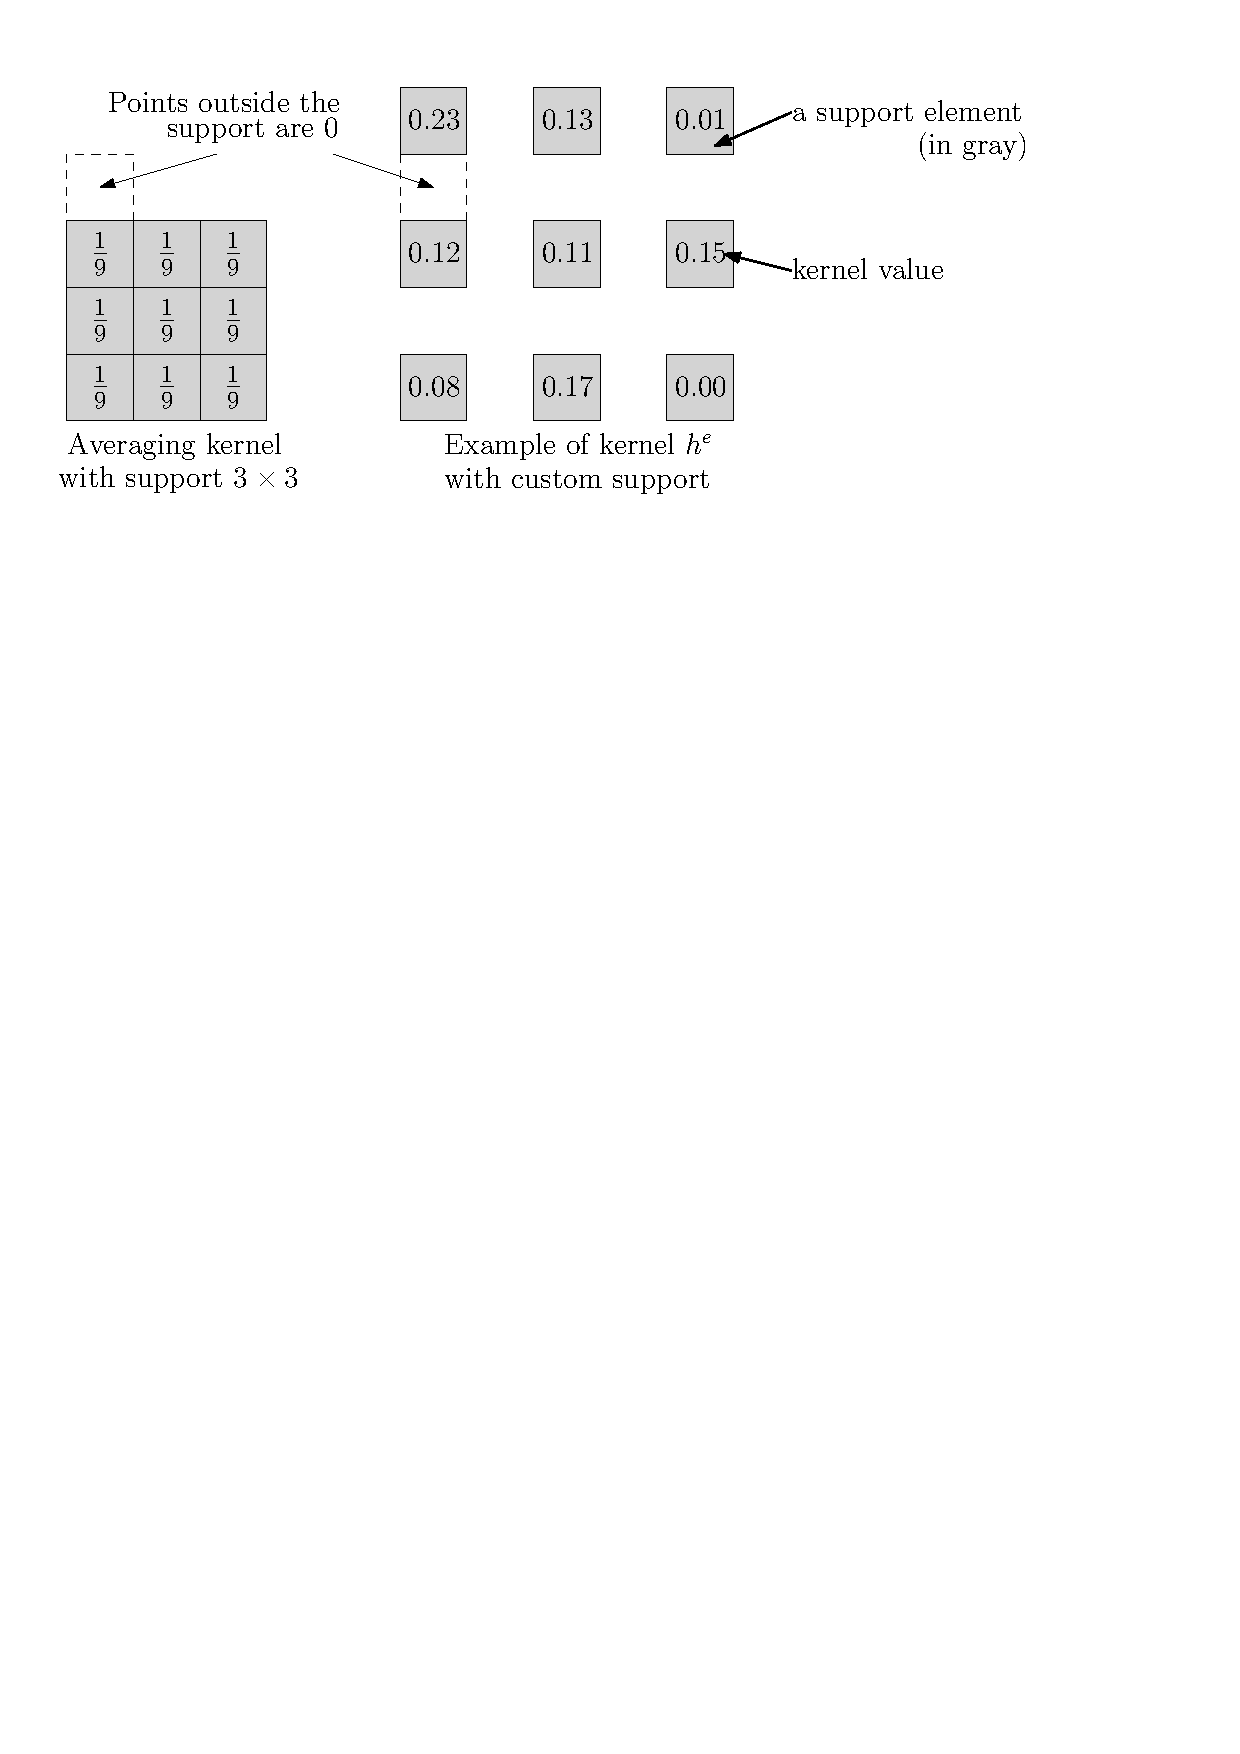
\includegraphics[width=0.8\textwidth]{figures/example-kernel.pdf}
\caption{(a) A well-known averaging kernel, which has fixed support ($3\times3$) and fixed values. (b) Example of a kernel $\h^e$. The locations of the gray squares and the values (e.g. $.01$) actually change during PALMTREE. The shape of this $\h^e$ (like a chessboard) has been shown experimentally to work well. \label{fig_example_kernel}}
\end{figure}

One column of the dictionary $\D$ corresponds to the convolution of successive kernels on a given branch identified by the leaf $l$. We will denote that successive convolution by
\begin{flalign*}
&& \h^{*l} = & \h^r * \dots * \h^l  && \text{$\triangleright$ atom $l$ of $\D$}
\end{flalign*}





Using the matrix notation, the dictionary-as-a-tree $\D$ applied to a code $\x$ approximates $\y$:


$$\D\x \approx \y$$

The code $\x$ belongs to $\mathbb{R}^{L\times N}$. $\D$ has dimensions $N \times L$ and $\y$ belongs to $\mathbb{R}^N$. 

Showing that $\D$ can be written as a matrix allows to compare the performance of PALMTREE against a simple matrix-vector product. Here is the "PALMTREE way" of computing $\D\x$:

\begin{align}
	\D\x = \sum_{l \in \L} \x^l * \h^{*l}	 \label{eq_Dx_as_convolution}
\end{align}

where $h^{*l}$ denotes the successive convolution of every kernel on the branch that leads to leaf $l$.



\section{The (FTL) problem}

The dictionary update step is defined as 
\begin{align}
(FTL) \quad \underset{\substack{(\h^e)_{e}}}\min ~ & \lVert \D\x - \y \rVert_2^2 \label{eq_ftl_energy}\\
\text{s.t.~} & \s^e_p=0 \Rightarrow \h^e_p = 0 \quad & \forall e \in \E, \forall p \in \P \label{eq_ftl_in_support} \\
 & \lVert \h^e \rVert \le \gamma & \forall e \in \E\label{eq_ftl_kernel_finite_nrj}
\end{align}

The constraint \ref{eq_ftl_in_support} guarantees that each kernel $\h^e$ only has non-zero values on its support $\s^e$. \ref{eq_ftl_kernel_finite_nrj} constrains the overall energy of every support to be finite and prevents a specific kernel to "explode".

(FTL) can be rewritten as an unconstrained problem, shifting the constraint spaces $(D^e)_{e \in \E}$ to the objective function using the characteristic function $\chi_{D^e}$ defined for one edge $e$:
$$\chi_{D_e}(\h^e) = \begin{cases} 0 &\text{ if } \h^e \in D^e \\ +\infty & \ \text{otherwise}\end{cases}$$

(FTL) becomes:

\begin{align}
(FTL) \quad \underset{\substack{(\h^e)_{e}}}\min ~ & \lVert \D\x - \y \rVert_2^2 + \sum_{e}\chi_{D_e} (\h^e)
\end{align}

\subsection{Interesting (FTL) properties}
$\D\x$ can be seen (in \cref{eq_Dx_as_convolution}) as a polynomial of degree $2\text{depth}(\T)$. This implies that it is possibly extremely non-convex although being infinitely differentiable.

$$\Phi((\h^e)_{e \in \E}) = \lVert \D\x-\y \rVert^2_2$$

The interesting thing is that $\Phi$ is differentiable when only one $\h^e$ varies. % TODO

% TODO \cref{proof_ftl_polynomial}) 
% TODO FTL is non-convex...

\subsection{PALMTREE, the algorithm for solving (FTL)}
% TODO explain PALMTREE

\section{Issues with PALMTREE algorithm}
As explained in \cite[p. 23]{chabiron_optimization_2016}, the main drawbacks to use this convolutional tree model for practical dictionary learning (as many other applications) are the hand-made parts of the model, leading to arbitrary and sub-optimal results. Among them are the design of the tree (degree, depth...) and the choice of the supports. % TODO "degree" not understandable
\subsection{Choice of the tree}
The paper chooses to use a fixed tree structure, meaning that the tree (degree, depth) has been created \emph{ad-hoc} on a per-experiment basis, trying to mimic the frequency pyramid tiling of a curvelet decomposition. The number of leaves wasalso specifically chosen to match the number of atoms that was generated on the target image.

But getting an actual adaptative dictionary update step implies that designing the tree is made optimally and as part of the optimization process. This is one of the internship research axis.

\subsection{Choice of the kernel supports}

As described in \ref{sec_tree_model}, the supports $\s^e$ are part of the dictionary-as-a-tree model. In \cite{chabiron_toward_2015}, the authors experimentally showed that using fixed supports for approximating curvelets is possible. For that specific purpose, the results turned to be good. But the whole model was supposed to be able to approximate any kind of image, hence the need for "adaptative" supports instead of hand-made ones. Figure \ref{fig_example_kernel} shows in dashed-line squares the hand-made support. The gray square show what we would expect from an "adaptive" support. Instead of keeping the same shape for every target atom, the supports evolves and get closer to the target shape.

And as for the tree design, the choice of where are located the elements of each kernel support has been made (so far) arbitrarily. The support of the $\h^e$ kernel of fig. \ref{fig_example_kernel} shows an example of typical layout chosen for the experiments in \cite{chabiron_optimization_2016}. 

But our goal is to be able to approximate any kind of atoms, as \ac{KSVD} is able to do. Being able to choose what elements should be in the kernel supports as part of the optimization process is another goal during this internship.

\begin{figure}[!ht] \centering
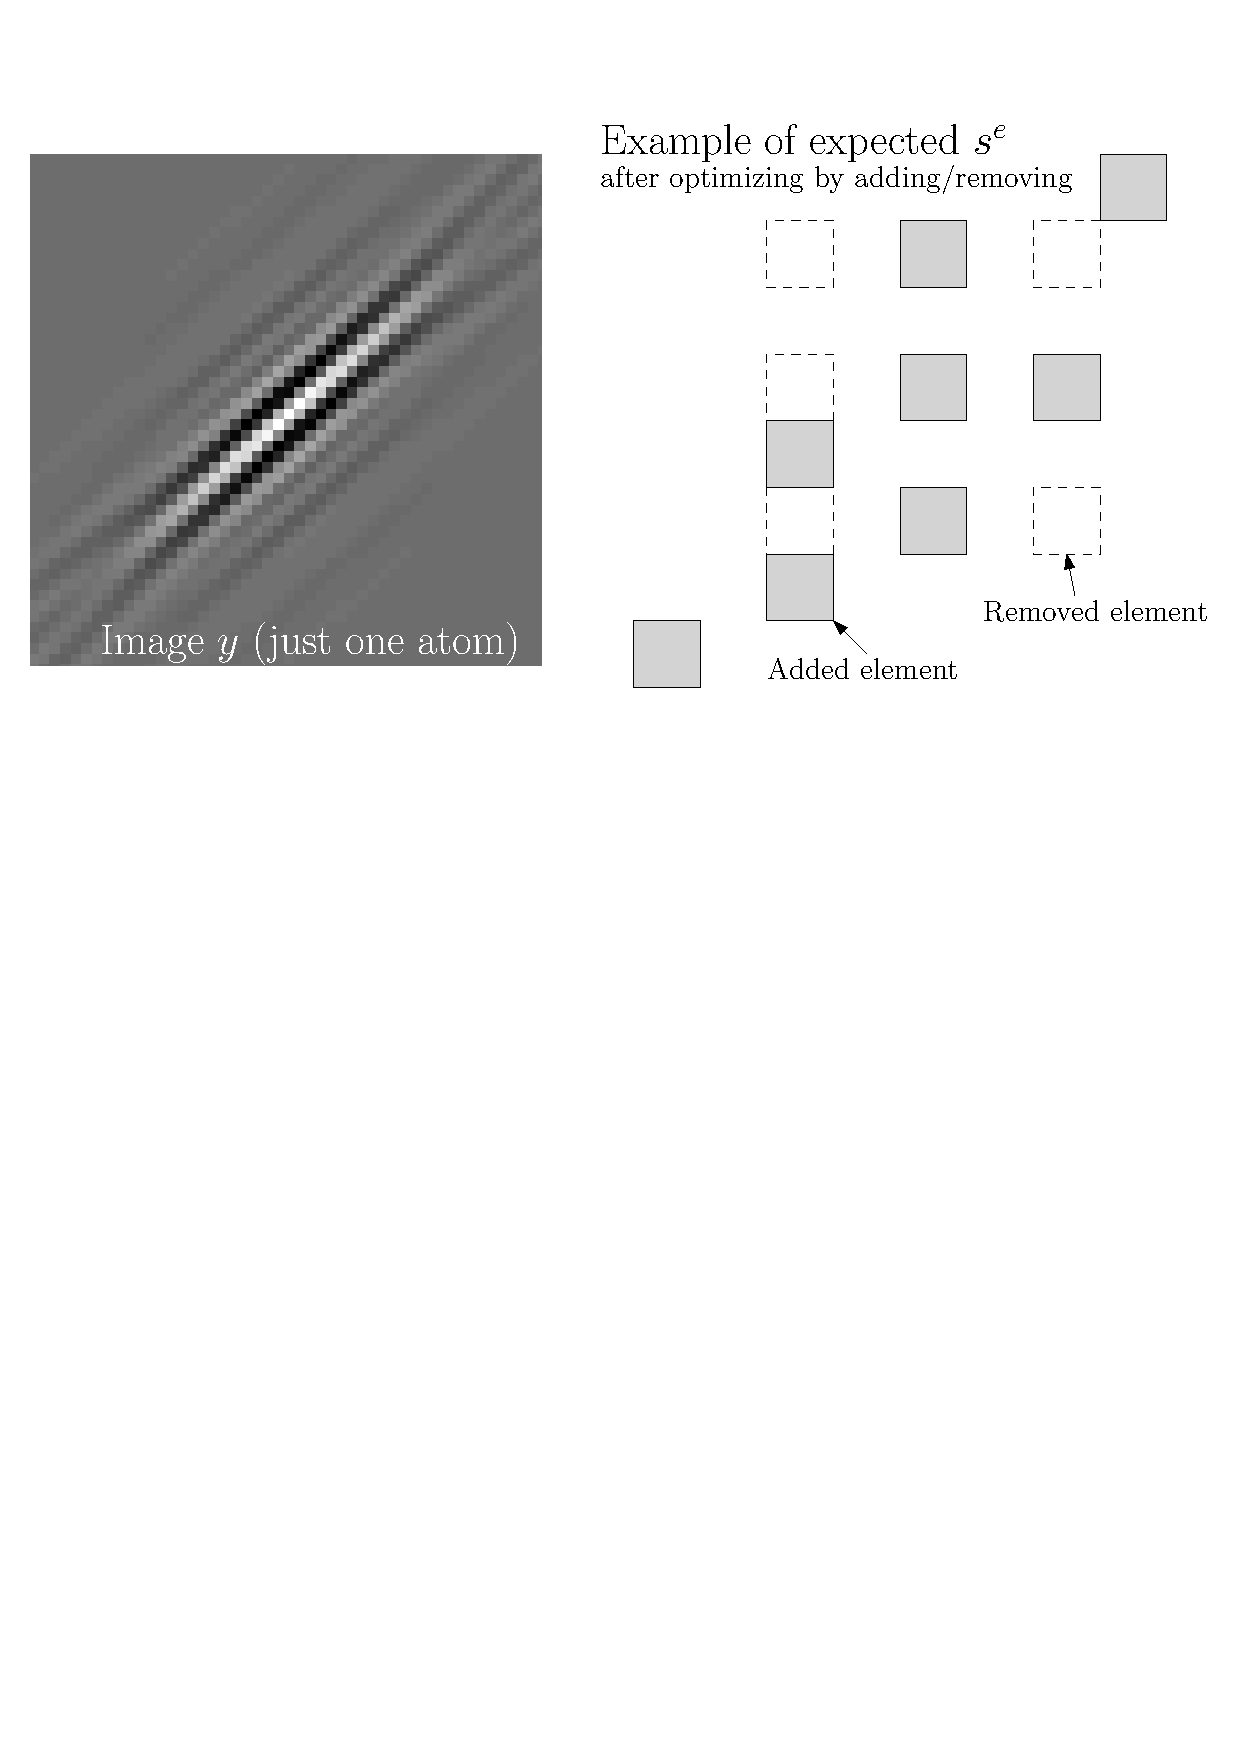
\includegraphics[width=0.6\textwidth]{figures/add-rm-elmts-support.pdf}
\caption{On the left, a simple curvelet atom which serves as target image. The right figure represents the locations of the support element for one of the kernels of the tree. The dashed squares represent the initial support given in figure \ref{fig_example_kernel}. The gray squares show the (supposedly) locations of the support elements after optimization. The elements have moved to the general direction of the curvelet.\label{fig_example_optimal_support}}
\end{figure}


\chapter{Experiments}

\section{First research axis: experimenting with adaptative supports}

After being able to correctly add and remove support elements, the second phase was to think about what elements we would add or remove, and when (i.e. when during the PALMTREE algorithm).

The figure \ref{fig_example_optimal_support} shows an example of what we think would happen when allowing to add and remove elements: the support would shape itself to better match the target atom (in fig.\ref{fig_example_optimal_support}, the atom shown is actually the whole target image).


\subsection{Adding an element}
Our first thought on how to add an element to a support was to find the best kernel among the tree edges, and then pick the best point(s) of that support to be added. We thought the gradient of the objective function would probably give that information. 

% TODO explain 






\section{Using the gradient for adding support elements}

The Orthogonal Matching Pursuit (OMP, detailed in \cref{alg_omp}) chooses which component $\x_i$ should be "turned on" at each iteration, finding the atom $d_i$ that has the greatest correlation with the residual $R$. This step (cf. \cref{alg_omp_pick_correlation}) uses the gradient $\nabla \Phi(\x)$, with $$\Phi(\x) = \lVert \D\x - \y \rVert^2$$


\begin{algorithm}[!ht]
    \caption{Orthogonal Matching Pursuit (OMP) algorithm for sparse approximation}\label{alg_omp}
  \begin{algorithmic}[0]
    \Input signal $\y$ of dimension $N$, dictionary of dim $N \times K$ with $K>>N$
    \Output A $k$-sparse code $\x$ of dimension $K$
    \State \textbf{Initialization} $\bm{r}^{(0)} = \y$, $I=\{\}$
    \While{$i \leq k$}
      \State $l =  \underset{l = 1,\dots,l}{\arg\max} | \nabla \Phi(\x) |$ \label{alg_omp_pick_correlation}\Comment{find atom with max. correlation with $R$}
      \State $S = S \cup \{l\}$
      \State $\x = \underset{supp(\x) \subset S}{\arg\max} \Phi(\x)$
      \State $\bm{r}^{(i+1)} = \bm{r}^{(i)}-\x_l d_l^{(i)}$
      \State $\hat{\y} = \hat{\y}+\langle \bm{r}^{(i)}, \d_{l}^{(i)} \rangle \d_{l}^{(i)}$
      \State $i = i + 1$
    \EndWhile
  \end{algorithmic}
\end{algorithm}

Our idea is to use the same principle when adding elements to supports $(\s^e)_{e \in \E}$: add a new element to one of the supports between two iterations of the PALMTREE algorithm, using the greatest gradient component information.

But is it actually correct to choose the element to be added using a strictly local information (the gradient)? Also, how to get the "full" gradient as the current gradient is only computed on the points of the support?

We will first review how the "full" gradient is computed and then describe a way to check that the gradient gives a good direction towards a critical point.

\subsection{Computing the "full" gradient}
Up to now, the gradient was computed using a convolution based on translations. It takes advantage of the sparsity of each kernel $\h^e$ as well as the fact that the proximal operator is projecting every kernel onto its support, meaning that only a few elements have to be computed.

We basically chose to use the fast Fourier transform ($\F$) for computing the convolution on the whole kernels:
\begin{align*}
	\nabla_{\h^f} \Phi((\h^e)_{e \in \E})&= \F^{-1}(\F(H^{e'})^* \text{.\^{}} \F(R))
\end{align*}
with ${}^*$ denoting the adjoint operator, $\text{.\^{}}$ the point-wise product, $H^{f}$ the (todo) % TODO H^e?

\subsection{Is the gradient right?}
We had some trouble when trying to compute the gradient on the full kernels $(\h^e)_{e \in \E}$ (not only on the supports element locations). To be sure that the computed "full" gradient was correct, we compared it to a finite-diffences gradient:

$$\lim_{\epsilon \rightarrow 0} \frac{\Phi((\h^e)_{e \in \E}+\epsilon e_i) - \Phi ((\h^e)_{e \in \E}) }{\epsilon} ~\overset{?}{=}~ \nabla_i \Phi ((\h^e)_{e \in \E})$$

\begin{figure}[!ht]\centering
\begin{subfigure}[b]{0.40\textwidth}\centering
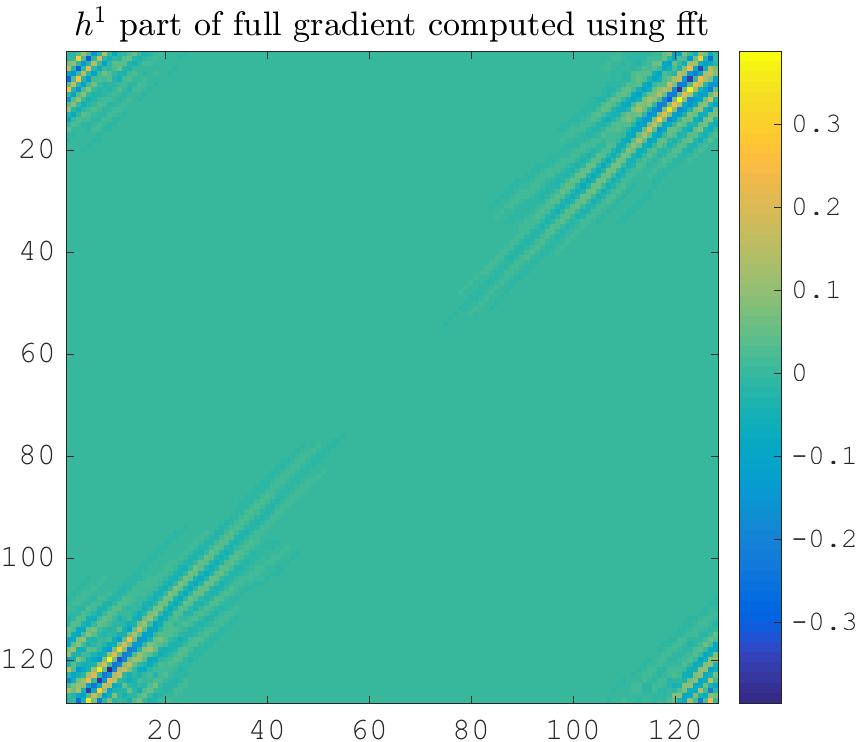
\includegraphics[width=\textwidth]{figures/verif_gradient/gradient.png}
\end{subfigure}
\begin{subfigure}[b]{0.40\textwidth}\centering
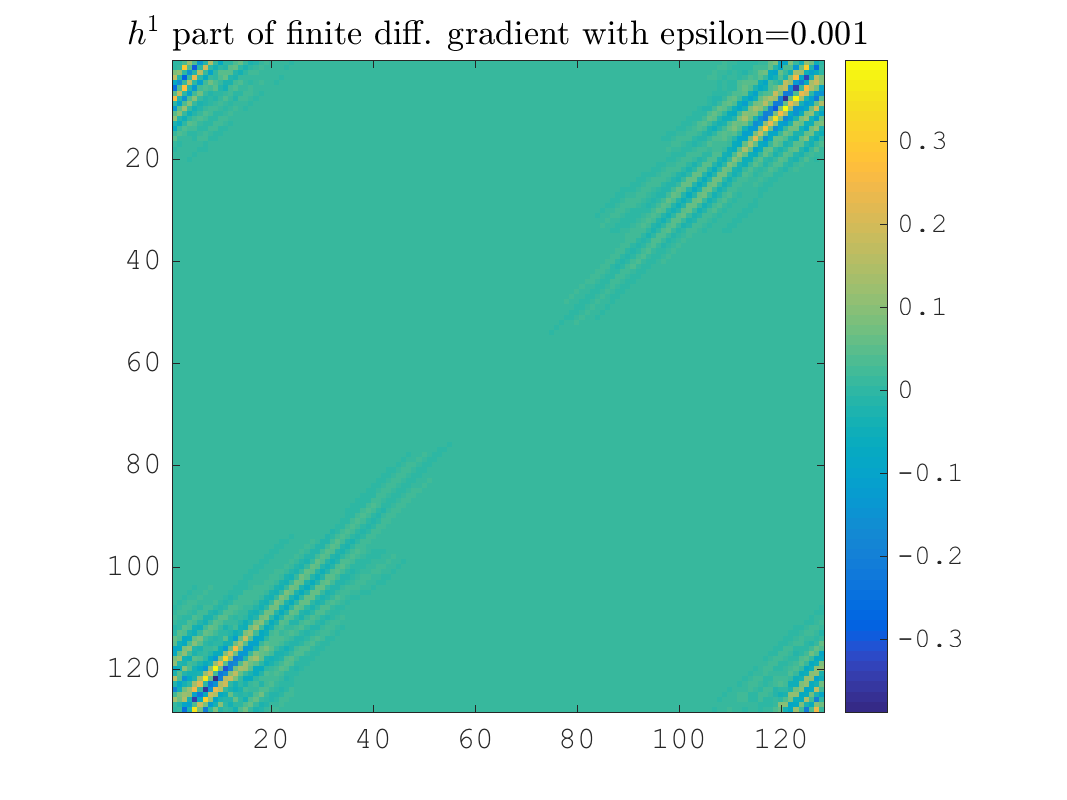
\includegraphics[width=\textwidth]{figures/verif_gradient/finite-diff.png}
\end{subfigure}
\begin{subfigure}[b]{0.40\textwidth}\centering
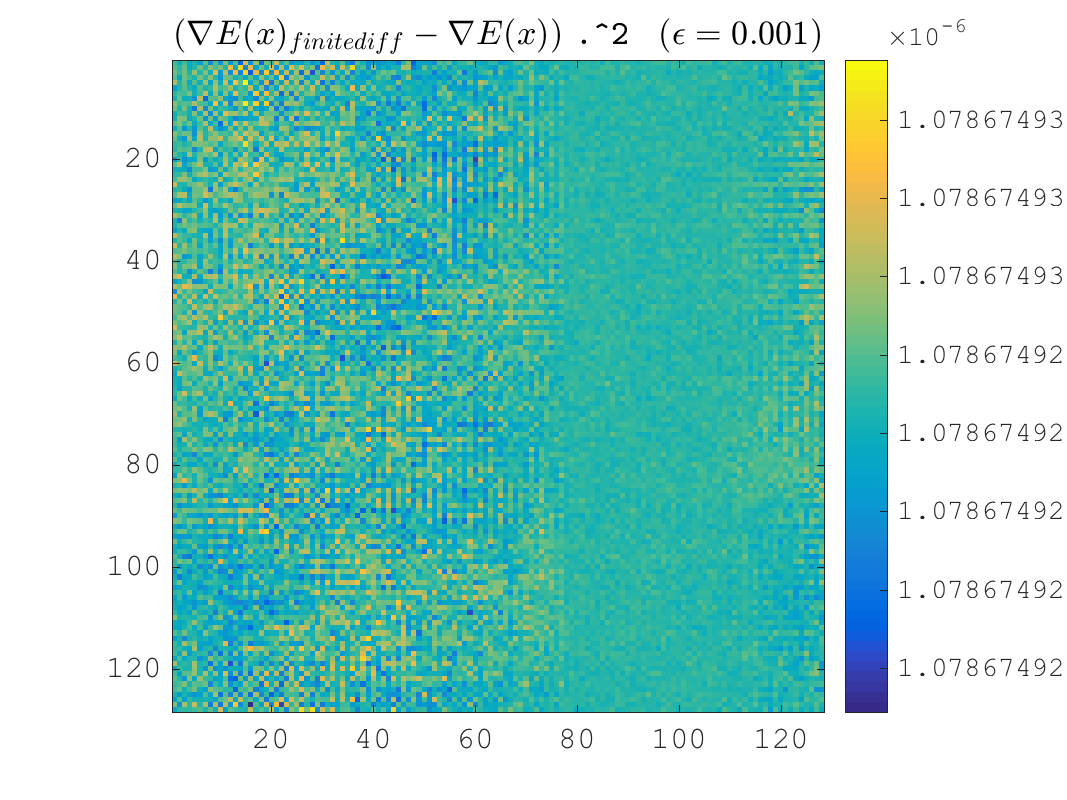
\includegraphics[width=1\textwidth]{figures/verif_gradient/rest.png}
\end{subfigure}
\begin{subfigure}[b]{0.40\textwidth}\centering
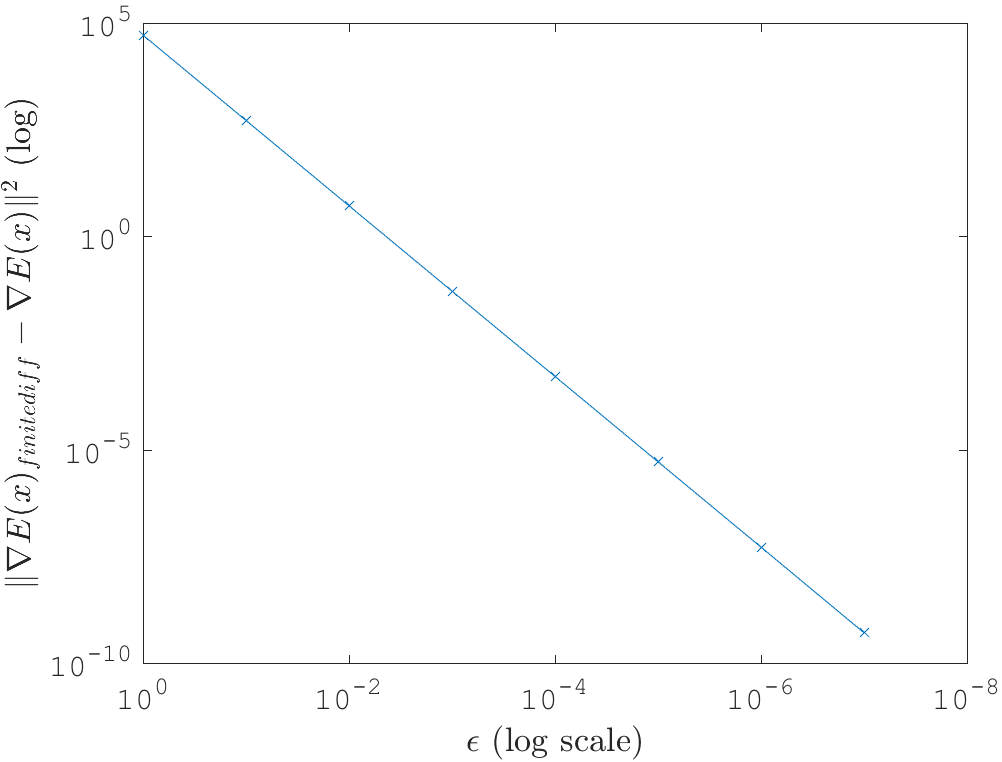
\includegraphics[width=1\textwidth]{figures/verif_gradient/finite-diff-vs-grad.png}
\end{subfigure}
\caption{Checking that the "full" gradient is correct. We compare it to the finite-difference gradient and make the $\epsilon$ tend to 0.} \label{fig_verif_gradient}
\end{figure}

Figure \ref{fig_verif_gradient} compares the FFT-computed gradient to the finite-differences gradient (with $\epsilon=0.001$). The bottom left figure shows that the two gradients are very close in term of difference. The right figure shows that the finite-differences gradient converges to the "full" gradient, which confirms that our "full" gradient is correct.

\subsection{The ideal elements to be added}\label{sec_gain_per_added_point}

One way to know if the "full" gradient leads to a good solution after many iterations, we designed the \cref{alg_gain_per_added_point} that tries every possible point added to one of the supports and see how much the objective function decreases. We named the resulting matrix \emph{gain-per-added-point} with the notation $\g^f$ ($f$ is edge of the studied support).

$\g^f$ represents for each point $p \in \P$ the minimized objective function if an element were added on support kernel $\s^f$ at that specific location (cf. \cref{alg_gain_per_added_point}).

\begin{algorithm}[!ht]
    \caption{Gain-per-added-point for the support $\s^f$} \label{alg_gain_per_added_point}
  \begin{algorithmic}[0]
    \Input One chosen edge $f$ and a tree $\T$
    \Output $\g^f$, the gain per added point for support $\s^f$
    \State $(\k^e)_{e \in \E} = \underset{(\h^e)_{e \in \E}}{\arg\min}~ \Phi ((\h^e)_{e \in \E})$ \quad s.t.~$\h^e \in D^e$ \quad $\forall e \in \E$ \Comment{common starting point}
    \For{each point $p \in \P$}
    	\State $\s^f_p = 1$ \Comment{add element to support}
    	\State $\g^f_p = \underset{(\k^e)_{e \in \E}}{\min}~ \Phi ((\k^e)_{e \in \E})$ \quad s.t.~$\k^e \in D^e$ \quad $\forall e \in \E$
    	\State $\s^f_p = 0$ \Comment{remove element to support}
    \EndFor
  \end{algorithmic}
\end{algorithm}

The figure \ref{fig_gain_vs_grad} compares (c) the gain-per-added-point of $s^4$ to (d) the absolute value of the partial gradient w.r.t $h^4$ after a full minimization. It is interesting to see that they share the same direction and shape. After selecting 20 of their best values in (e) and (f), we notice that they almost match, which reinforces our hypothesis that the gradient could give the right information for widening supports.

\begin{figure}[!ht]\centering
\begin{subfigure}[b]{0.49\textwidth}\centering
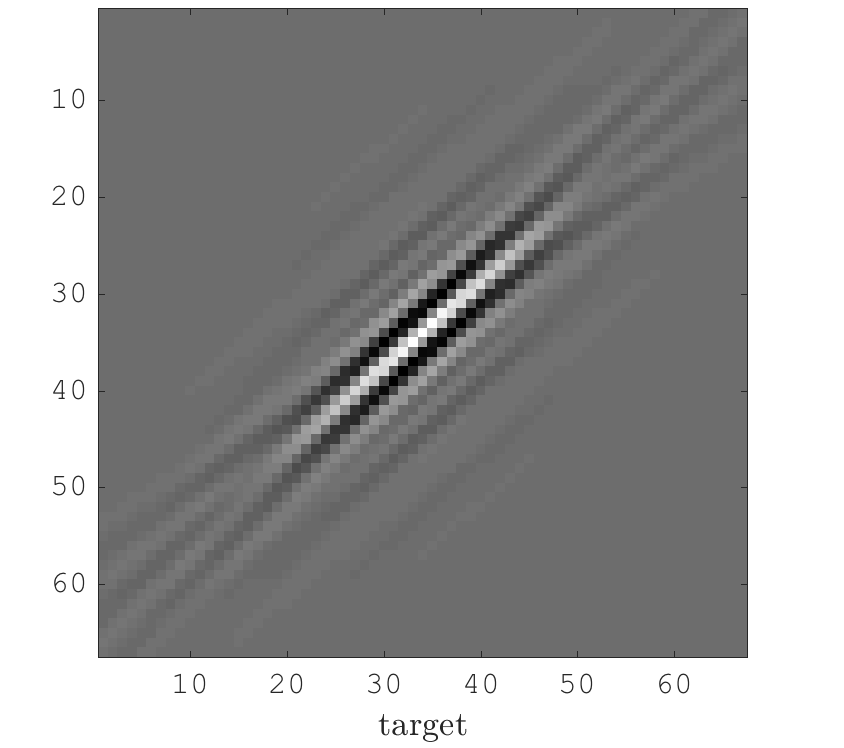
\includegraphics[width=\textwidth]{figures/xp/xp_128x128_sc2_angl1_K3_S3_node4_target.png}
\caption{Target}
\end{subfigure}
\begin{subfigure}[b]{0.49\textwidth}\centering
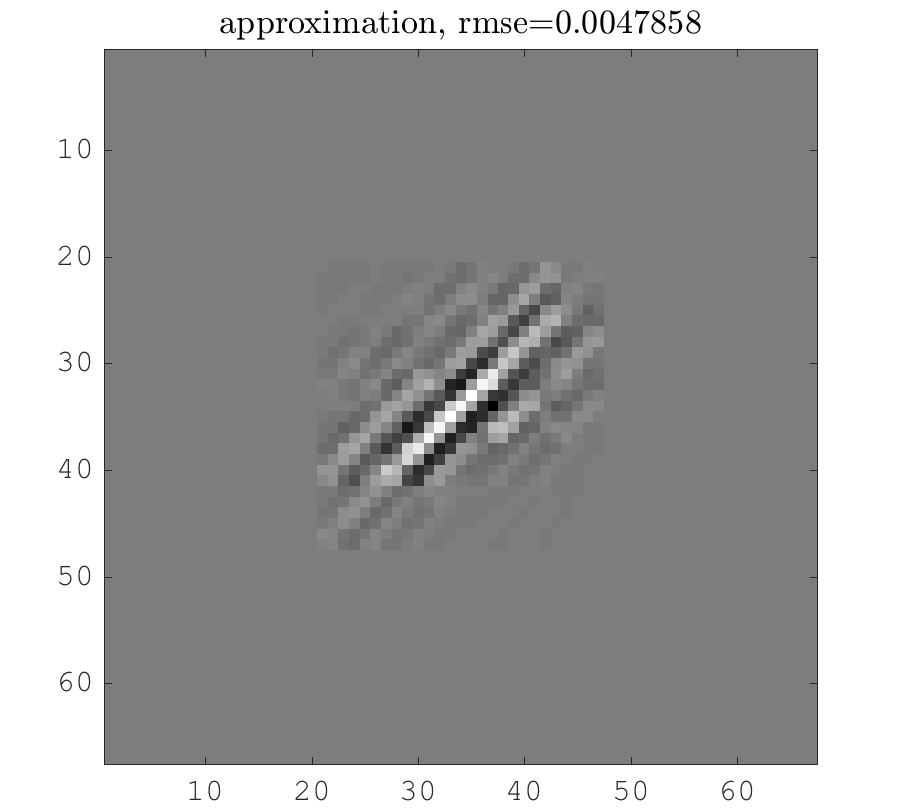
\includegraphics[width=\textwidth]{figures/xp/xp_128x128_sc2_angl1_K3_S3_node4_approx.png}
\caption{Approximation} \label{fig_gain_vs_grad_approx}
\end{subfigure}
\begin{subfigure}[b]{0.49\textwidth}\centering
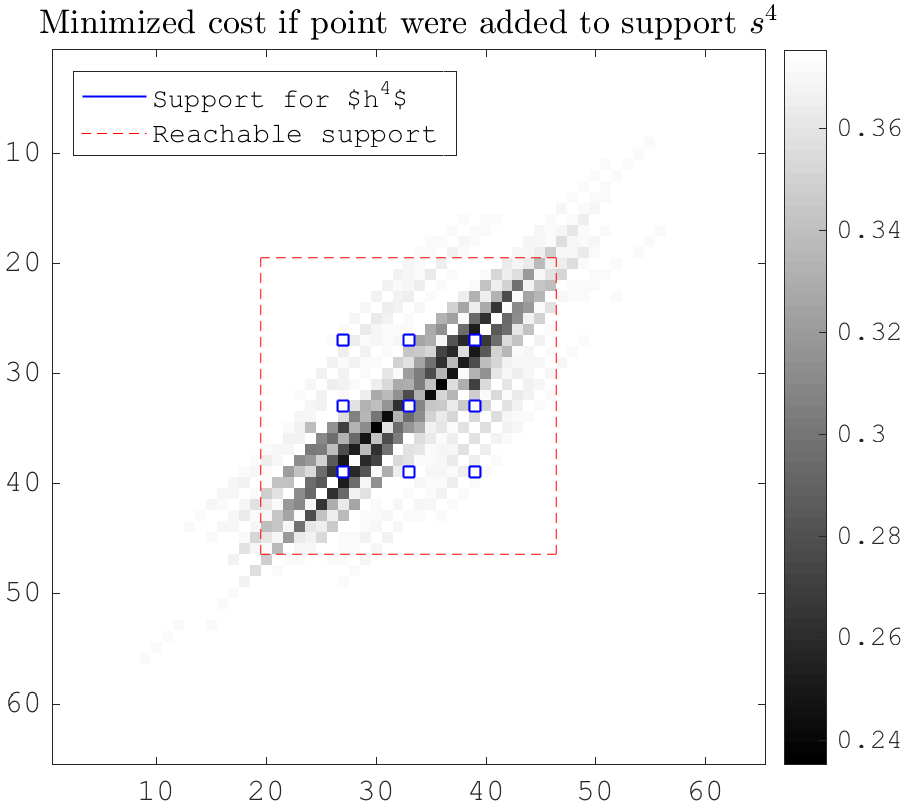
\includegraphics[width=\textwidth]{figures/xp/xp_128x128_sc2_angl1_K3_S3_node4_objmatrix.png}
\caption{Gain-per-added-point for $s^4$}
\end{subfigure}
\begin{subfigure}[b]{0.49\textwidth}\centering
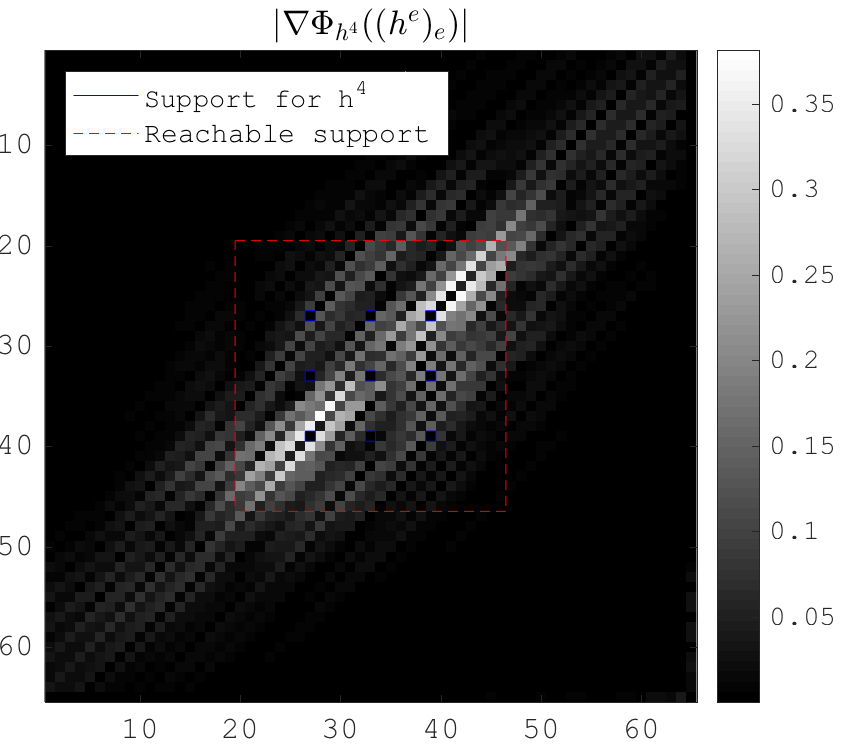
\includegraphics[width=\textwidth]{figures/xp/xp_128x128_sc2_angl1_K3_S3_node4_partgrad4.png}
\caption{Partial gradient w.r.t $h^4$}
\end{subfigure}
\begin{subfigure}[b]{0.49\textwidth}\centering
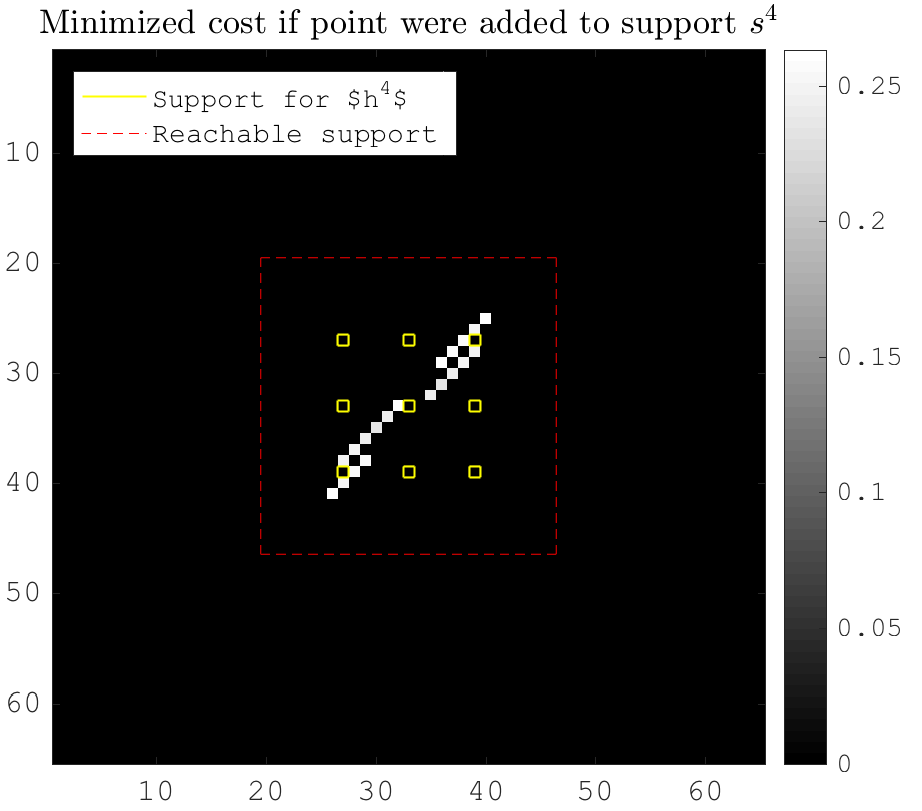
\includegraphics[width=\textwidth]{figures/xp/xp_128x128_sc2_angl1_K3_S3_node4_objmatrix_bestvalues.png}
\caption{Best values of above figure}
\end{subfigure}
\begin{subfigure}[b]{0.49\textwidth}\centering
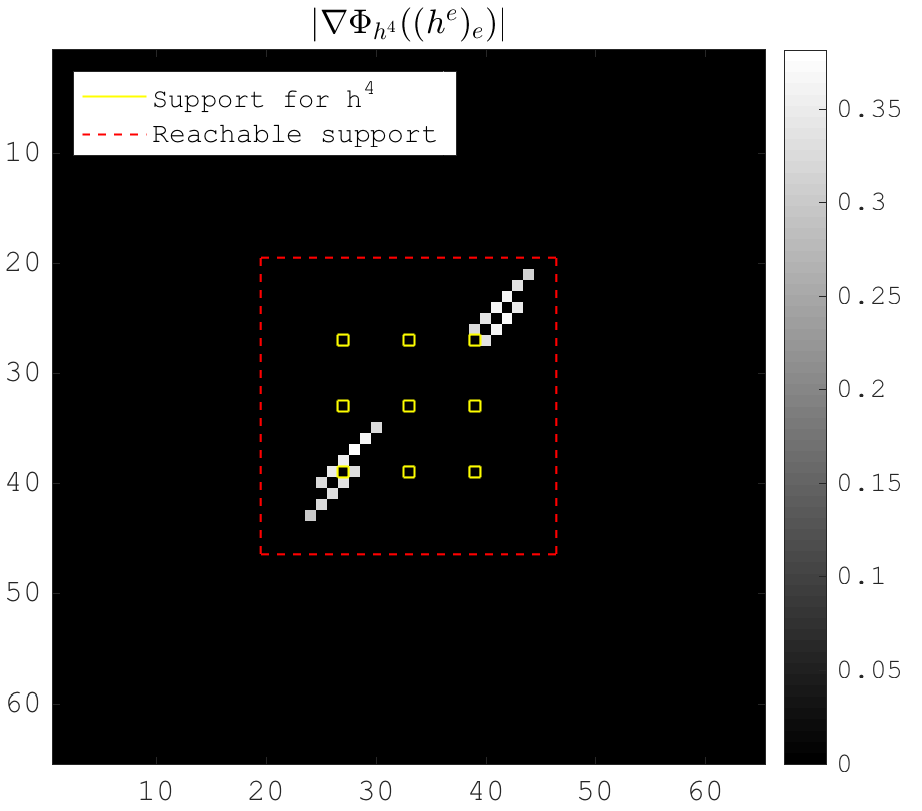
\includegraphics[width=\textwidth]{figures/xp/xp_128x128_sc2_angl1_K3_S3_node4_partgrad4_bestvalues.png}
\caption{Best values of above figure}
\end{subfigure}
\caption{Minimization of a single branch tree with fixed supports. This experiment uses a single-branch tree with 4 kernels.}\label{fig_gain_vs_grad}
\end{figure}

\subsection{Visual gain when adding an element}

\begin{figure}[!ht]\centering
\begin{subfigure}[b]{0.99\textwidth}\centering
	\begin{subfigure}[b]{0.32\textwidth}\centering
	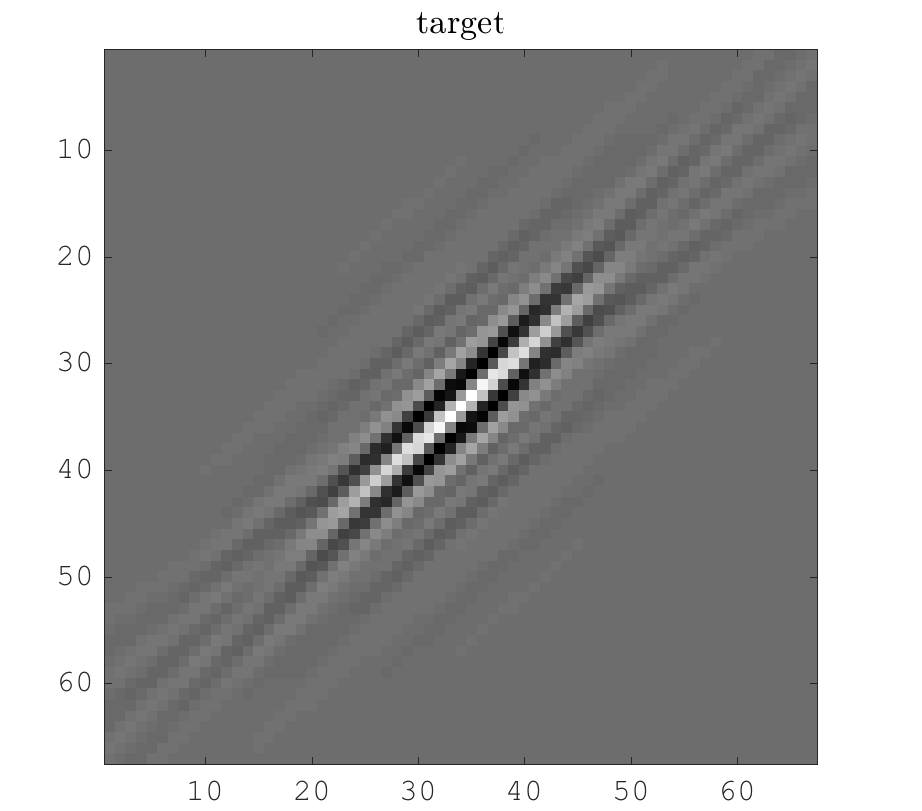
\includegraphics[width=\textwidth]{figures/before_after/xp_128x128_sc2_angl1_K3_S3_node4before_target.png}
		\caption{Target image}
	\end{subfigure}
	\begin{subfigure}[b]{0.32\textwidth}\centering
	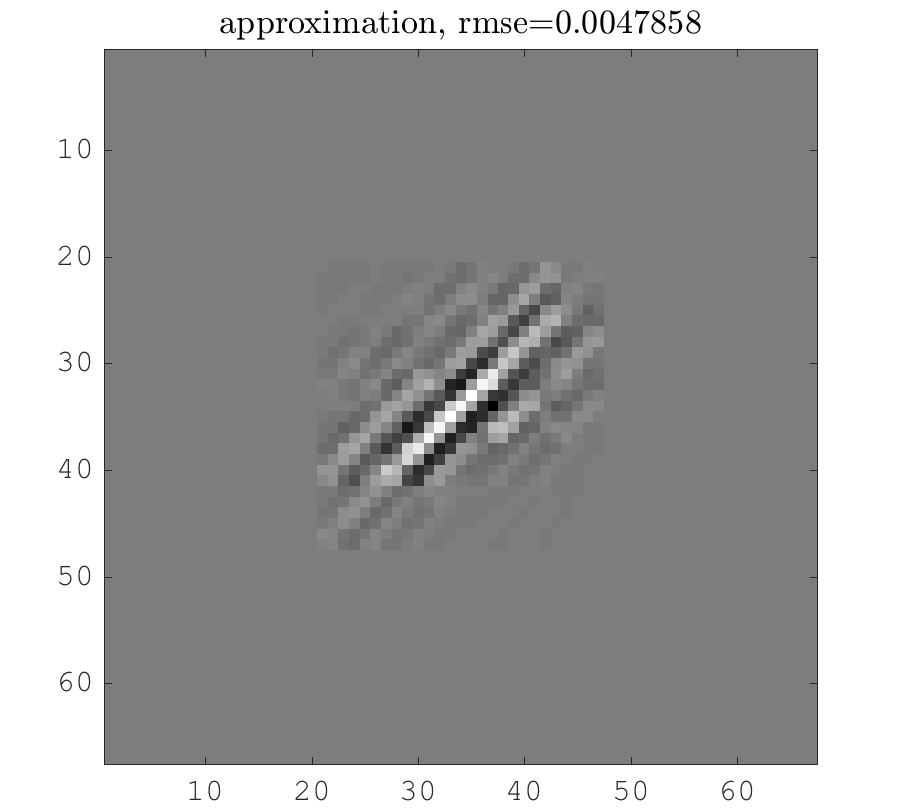
\includegraphics[width=\textwidth]{figures/before_after/xp_128x128_sc2_angl1_K3_S3_node4before_approx.png}
	\caption{Before adding}
	\end{subfigure}
	\begin{subfigure}[b]{0.32\textwidth}\centering
	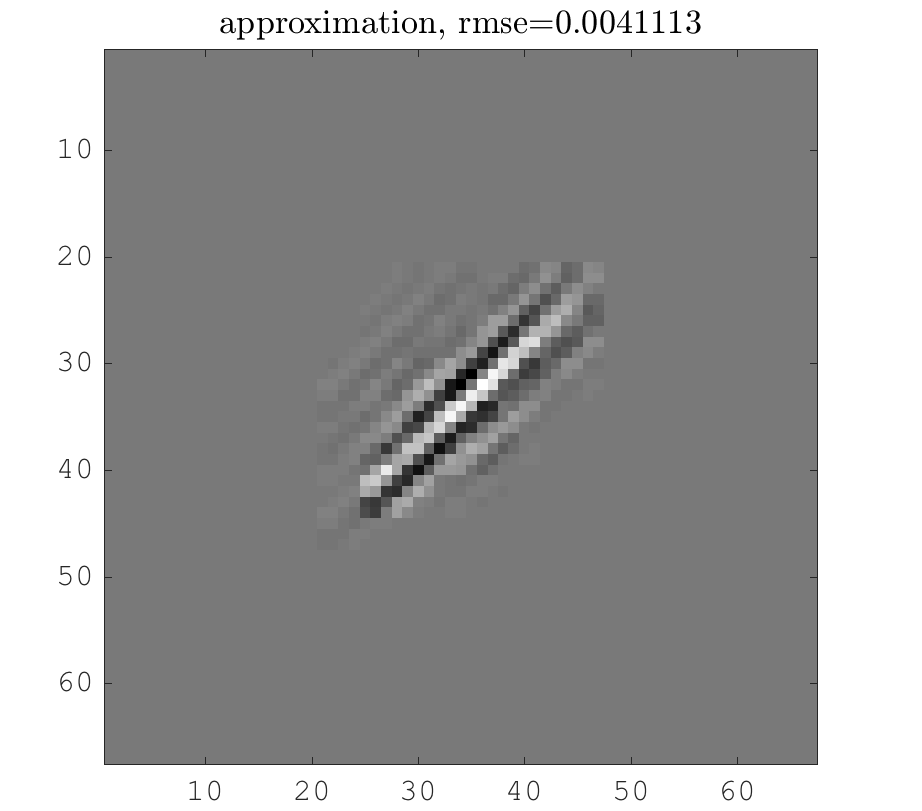
\includegraphics[width=\textwidth]{figures/before_after/xp_128x128_sc2_angl1_K3_S3_node4after_approx.png}
	\caption{After adding}
	\end{subfigure}
\end{subfigure}
\begin{subfigure}[b]{0.32\textwidth}\centering
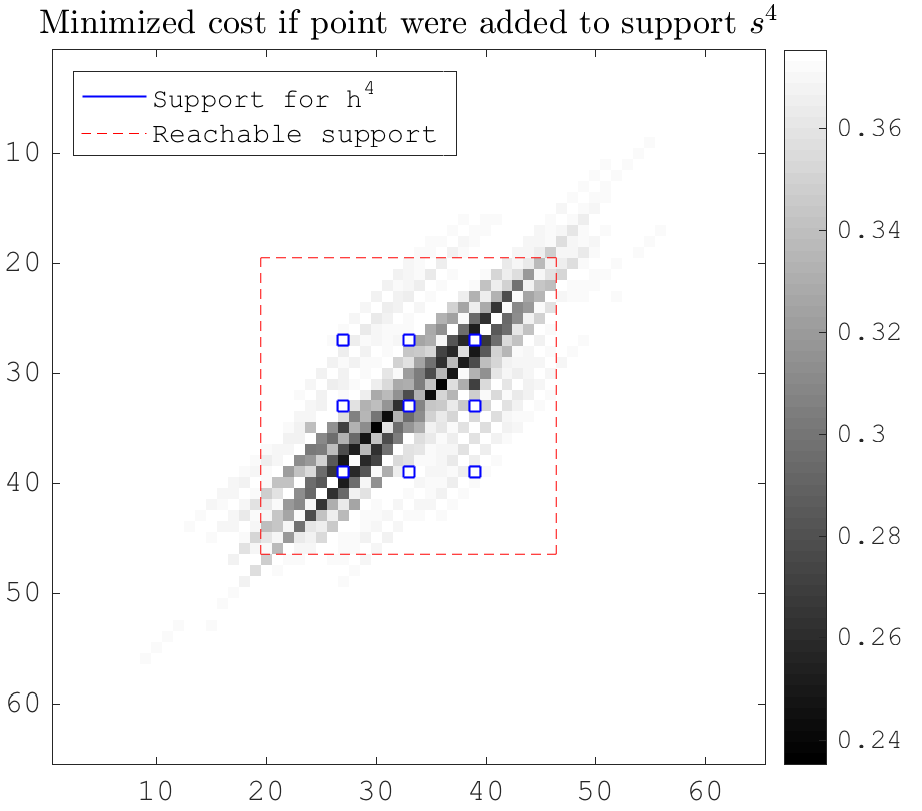
\includegraphics[width=\textwidth]{figures/before_after/xp_128x128_sc2_angl1_K3_S3_node4before_objmatrix.png}
\caption{Gain-per-added-point matrix} \label{fig_gain_matrix}
\end{subfigure}
\begin{subfigure}[b]{0.32\textwidth}\centering
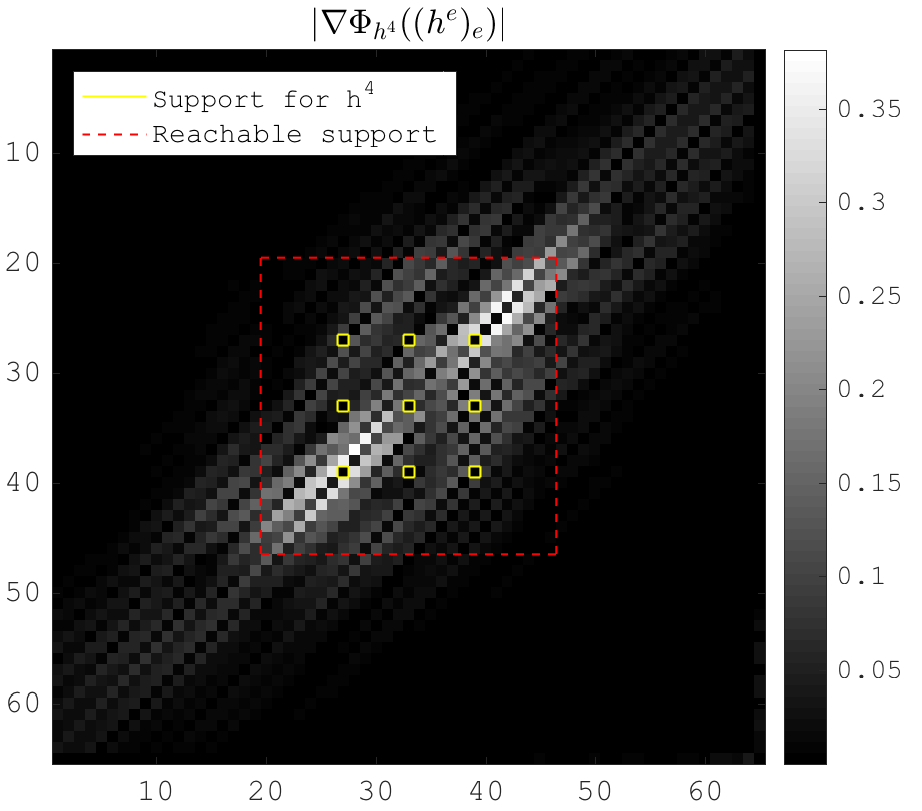
\includegraphics[width=\textwidth]{figures/before_after/xp_128x128_sc2_angl1_K3_S3_node4before_partgrad4.png}
\caption{Gradient before} \label{fig_grad_before}
\end{subfigure}
\begin{subfigure}[b]{0.32\textwidth}\centering
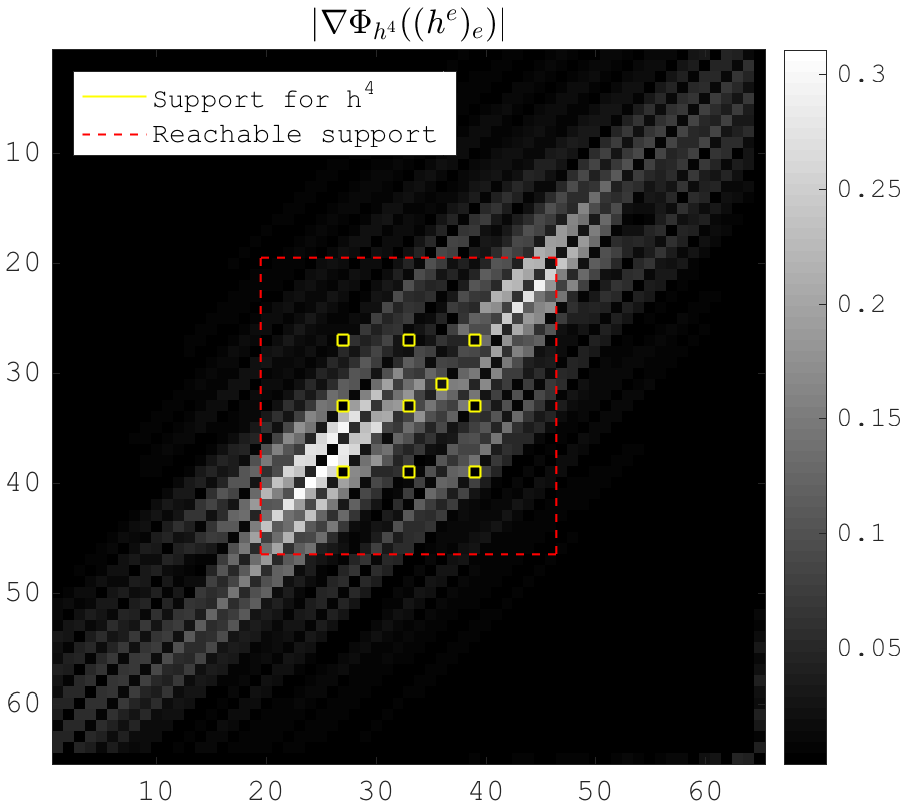
\includegraphics[width=\textwidth]{figures/before_after/xp_128x128_sc2_angl1_K3_S3_node4after_partgrad4.png}
\caption{Gradient after} \label{fig_grad_after}
\end{subfigure}
\begin{subfigure}[b]{0.32\textwidth}\centering
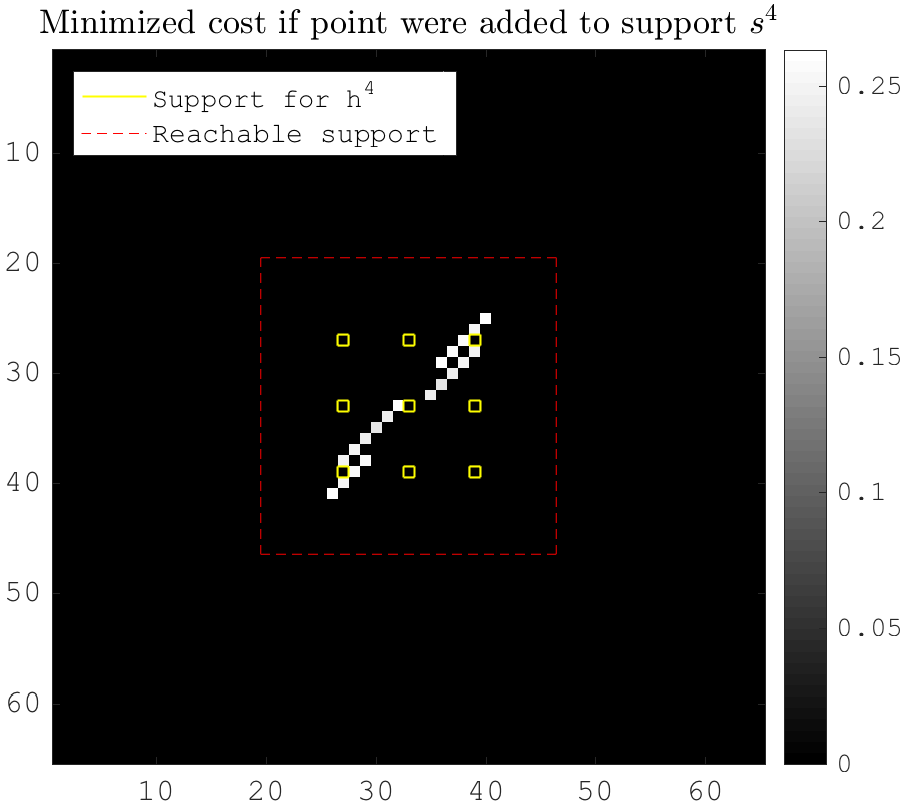
\includegraphics[width=\textwidth]{figures/before_after/xp_128x128_sc2_angl1_K3_S3_node4before_objmatrix_bestvalues.png}
\caption{Best values of \ref{fig_gain_matrix}}
\end{subfigure}
\begin{subfigure}[b]{0.32\textwidth}\centering
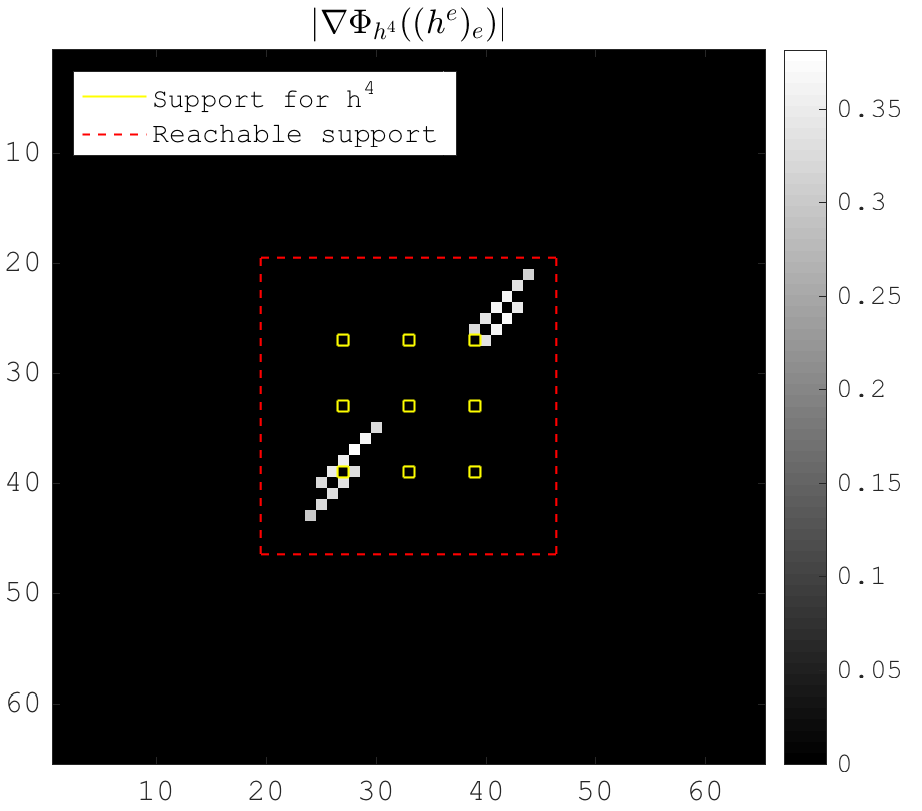
\includegraphics[width=\textwidth]{figures/before_after/xp_128x128_sc2_angl1_K3_S3_node4before_partgrad4_bestvalues.png}
\caption{Best values of \ref{fig_grad_before}}
\end{subfigure}
\begin{subfigure}[b]{0.32\textwidth}\centering
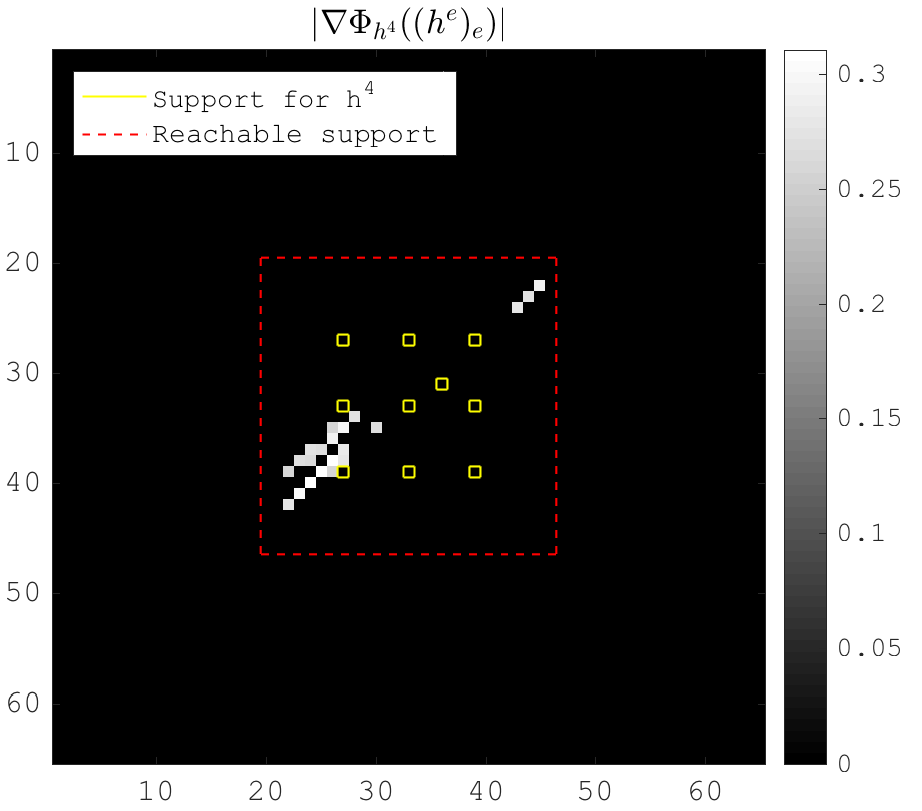
\includegraphics[width=\textwidth]{figures/before_after/xp_128x128_sc2_angl1_K3_S3_node4after_partgrad4_bestvalues.png}
\caption{Best values of \ref{fig_grad_after}}
\end{subfigure}
\caption{Effect of adding one point to the support $s^4$. The "before" tree is already minimized. The "after" tree has been added a point where the gain-per-added-point matrix were minimal.} \label{fig_before_after_adding}
\end{figure}

The experiment shown in \cref{fig_before_after_adding} is based on the results of \cref{fig_gain_vs_grad_approx}, where figures (a,b,d,e,g,h) are the same as the previous experiment. The figures (c,j,i) show what  happens if we add the minimum point of gain-per-added-point to $s^4$ and continue the minimization.

In the "before" gradient (\cref{fig_grad_before}) every point of the support (the small squares) has a null gradient: in the direction of those nine points, the gradient is null, meaning that we are at an critical point.

We can observe that adding a point to the support (materialized by the \nth{10} small square), the highest gradient values "shift" to the south-west. Adding a point to the support has an effect on every surrounding points.

\subsection{Local versus far away information}

The experiment in \cref{fig_gain_vs_grad} has only been done on a fully minimized tree, meaning that the gain-per-added-point would be "close" to what the gradient would indicate. But we could wonder if the gradient stays the same throughout all iterations; compared to the converged gain-per-added-point which is a "far away" information, the gradient might not lead to that gain.

The experiment shown in \cref{fig_iter_gain_vs_grad} compares the best values of gain-per-added-point to gradients snapshots taken during the minimization. This is reassuring: whatever the iteration, the gradient best values keep close to the gain-per-added-point best values.

\begin{figure}[!ht]\centering
\begin{subfigure}[b]{0.49\textwidth}\centering
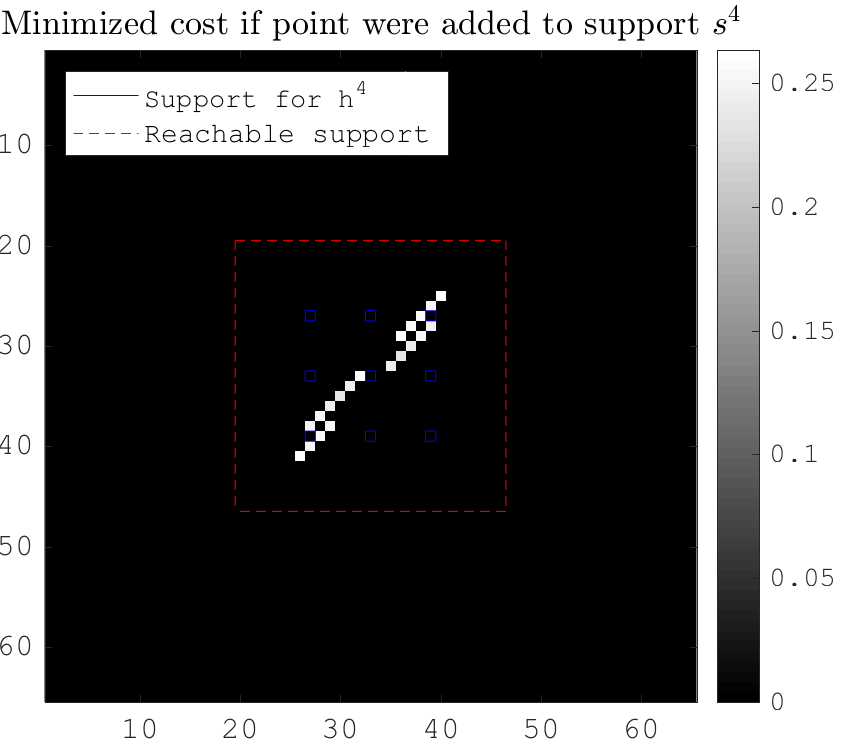
\includegraphics[width=\textwidth]{figures/xp_grad_iterations/xp_128x128_sc2_angl1_K3_S3_node4_objmatrix_bestvalues.png}
\caption{Gain-per-added-point matrix}
\end{subfigure}
\begin{subfigure}[b]{0.49\textwidth}\centering
	\begin{subfigure}[b]{0.49\textwidth}\centering
	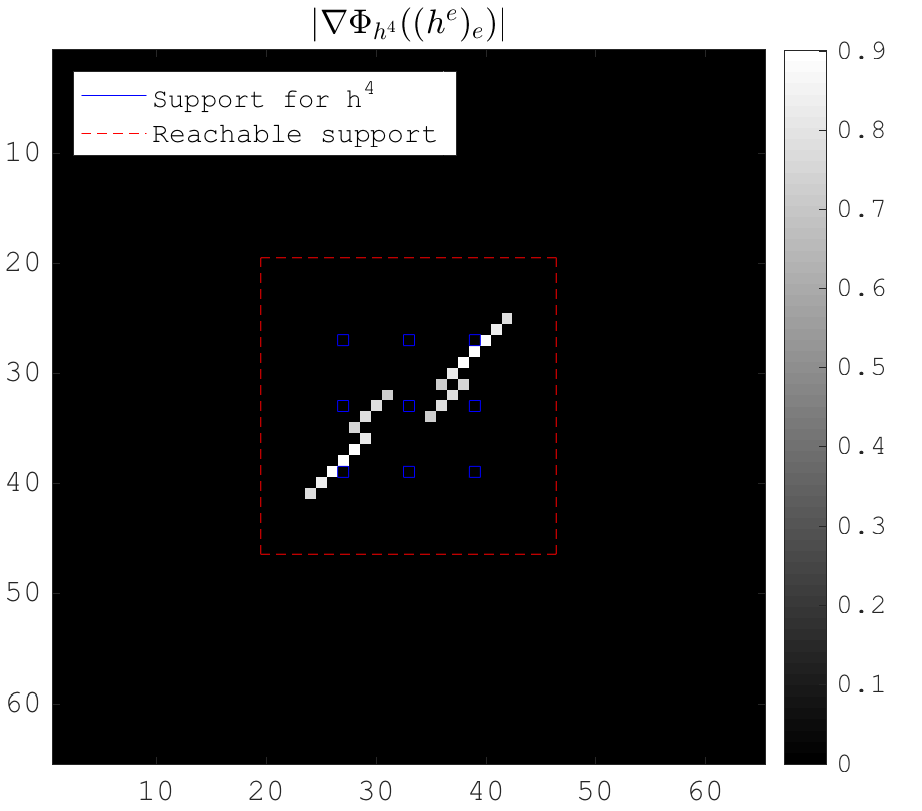
\includegraphics[width=\textwidth]{figures/xp_grad_iterations/xp_128x128_sc2_angl1_K3_S3_node4_1thiteration_partgrad4_bestvalues.png}
	\caption{Grad. iter. 1}
	\end{subfigure}
	\begin{subfigure}[b]{0.49\textwidth}\centering
	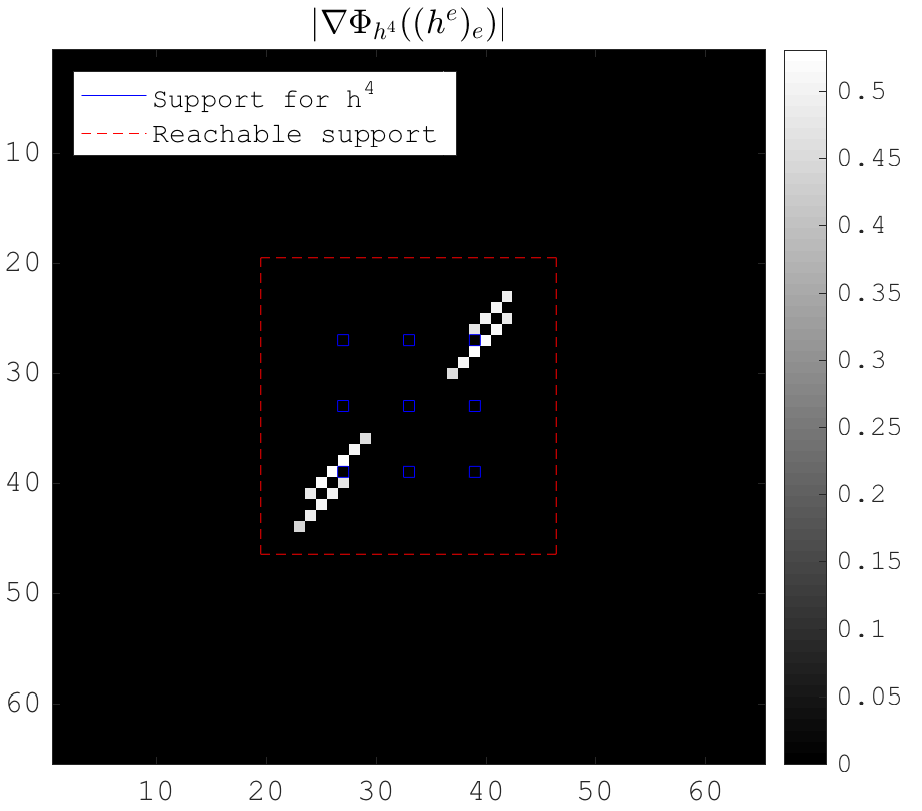
\includegraphics[width=\textwidth]{figures/xp_grad_iterations/xp_128x128_sc2_angl1_K3_S3_node4_8thiteration_partgrad4_bestvalues.png}
	\caption{Grad. iter. 8}
	\end{subfigure}
	\begin{subfigure}[b]{0.49\textwidth}\centering
	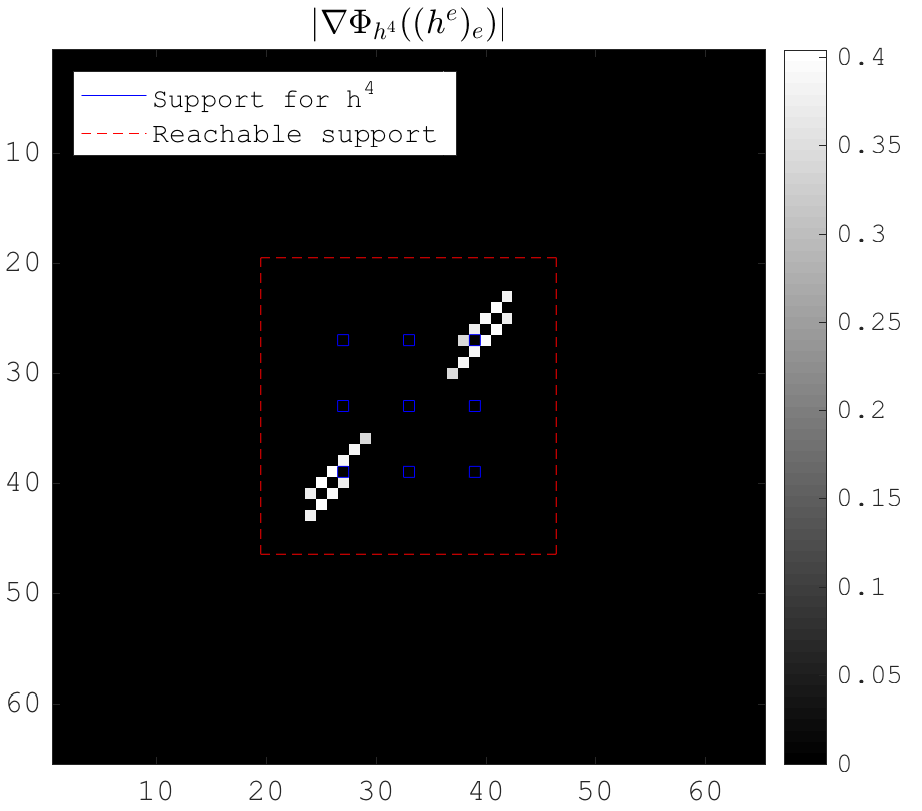
\includegraphics[width=\textwidth]{figures/xp_grad_iterations/xp_128x128_sc2_angl1_K3_S3_node4_20thiteration_partgrad4_bestvalues.png}
	\caption{Grad. iter. 20}
	\end{subfigure}
	\begin{subfigure}[b]{0.49\textwidth}\centering
	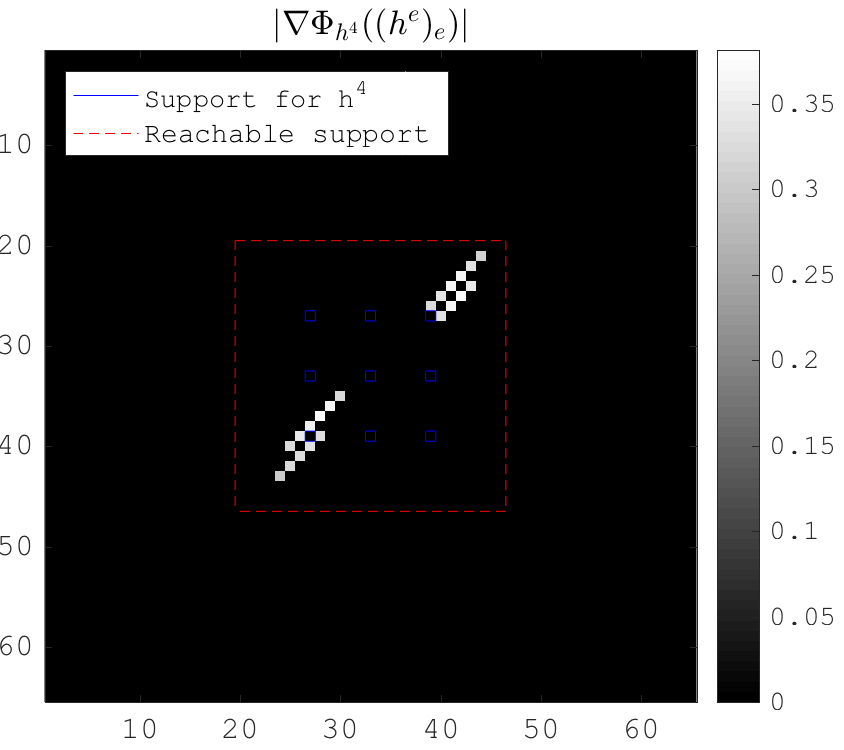
\includegraphics[width=\textwidth]{figures/xp_grad_iterations/xp_128x128_sc2_angl1_K3_S3_node4_partgrad4_bestvalues.png}
	\caption{Grad. iter. 200}
	\end{subfigure}
\end{subfigure}
\caption{Is the gradient giving the same information depending on the iteration? The conditions are the same as \cref{fig_simple_approx}. Only the best values are displayed.}\label{fig_iter_gain_vs_grad}
\end{figure}




\begin{figure}[!ht]\centering
\begin{subfigure}[b]{0.4\textwidth}\centering
	\begin{subfigure}[b]{1\textwidth}\centering
	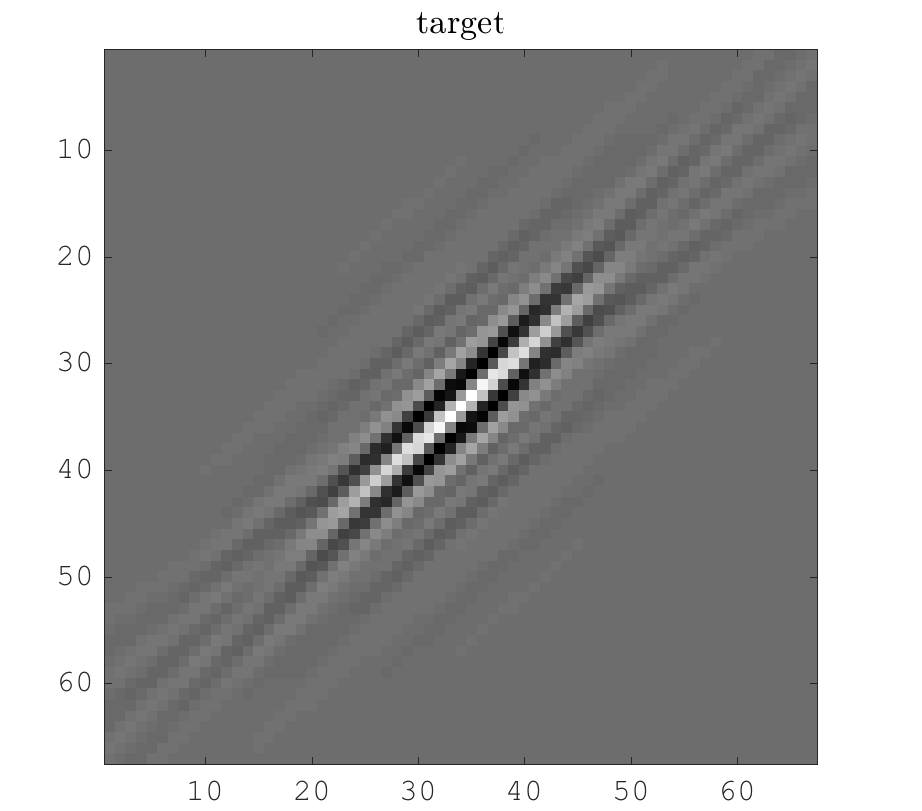
\includegraphics[width=\textwidth]{figures/variable_support/xp_128x128_sc2_angl1_K3_S3_node4_variable_support_target.png}
	\end{subfigure}
	\begin{subfigure}[b]{1\textwidth}\centering
	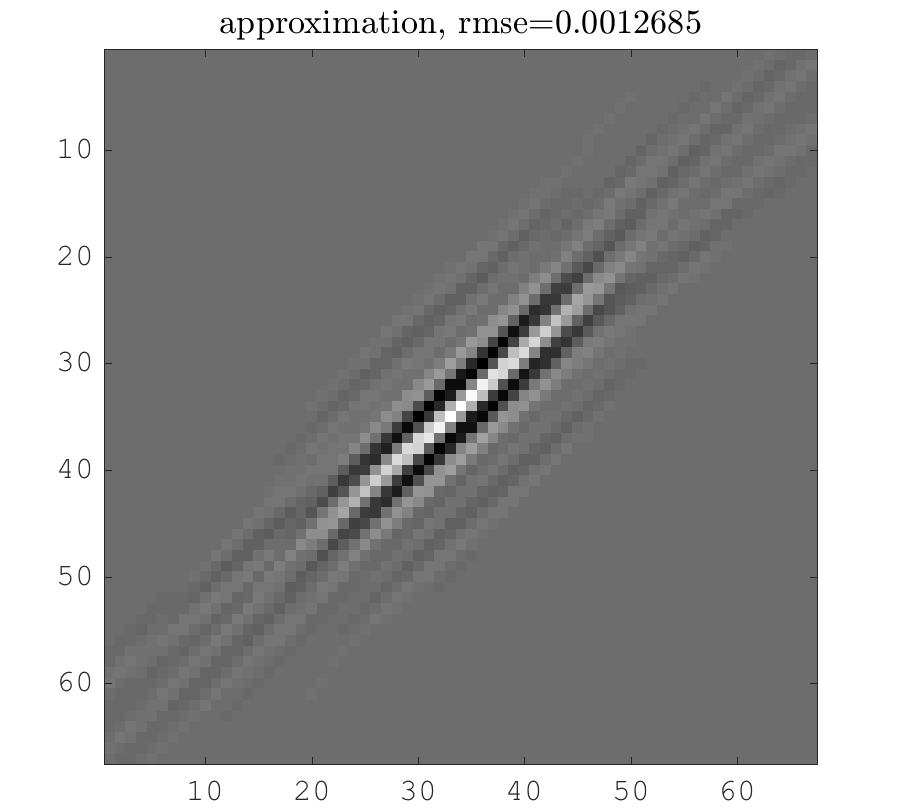
\includegraphics[width=\textwidth]{figures/variable_support/xp_128x128_sc2_angl1_K3_S3_node4_variable_support_approx.png}
	\end{subfigure}
\end{subfigure}
\begin{subfigure}[b]{0.4\textwidth}\centering
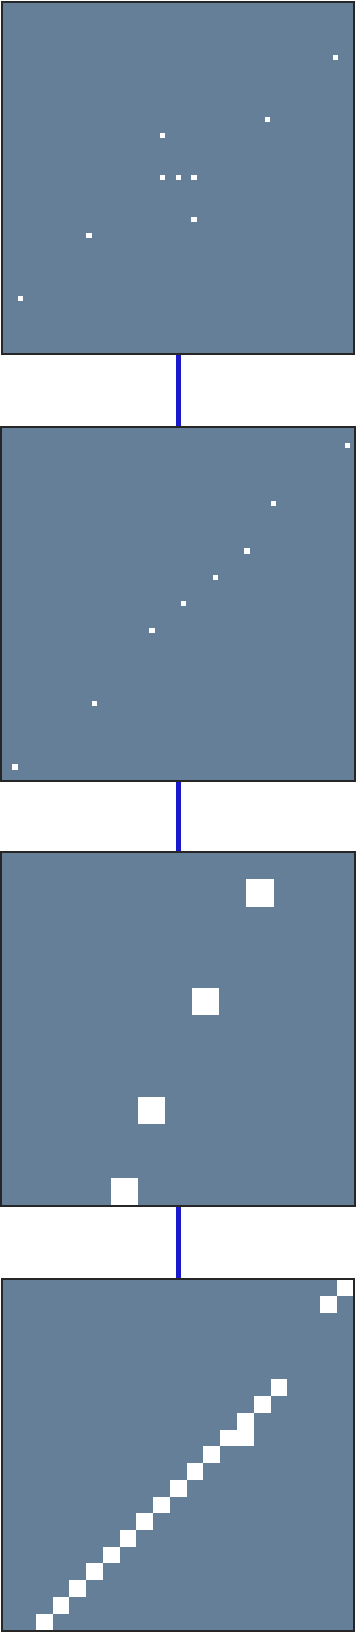
\includegraphics[width=0.37\textwidth]{figures/variable_support/support.pdf}
\end{subfigure}
\caption{Minimization using a variable support. Starting from simple diracs, the best element (using greatest gradient) is added to one of the supports every 5 iterations, up to 36 elements (same number as the fixed support in \cref{fig_single_branch}).} \label{fig_variable_support}
\end{figure}







\clearpage
\addcontentsline{toc}{chapter}{Appendix}
\appendix

\chapter{Miscellaneous}
\section{Link between convolutional tree and matrix $\D$}

Figure \ref{fig_block_circular} outlines the relation between the tree and the matrix form. The dictionary can be written using the notation

$$\D = \begin{bmatrix}C^5 & C^6\end{bmatrix} \begin{bmatrix}C^1 & C^2 & 0 & 0 \\0 & 0 & C^3 & C^4\end{bmatrix}$$
with $C^i$ the block-circular matrix for $\h^i$; it represents the final convolution $\h^{*l}*\x^l$ when using matrices.

\begin{figure}[!ht] \centering
	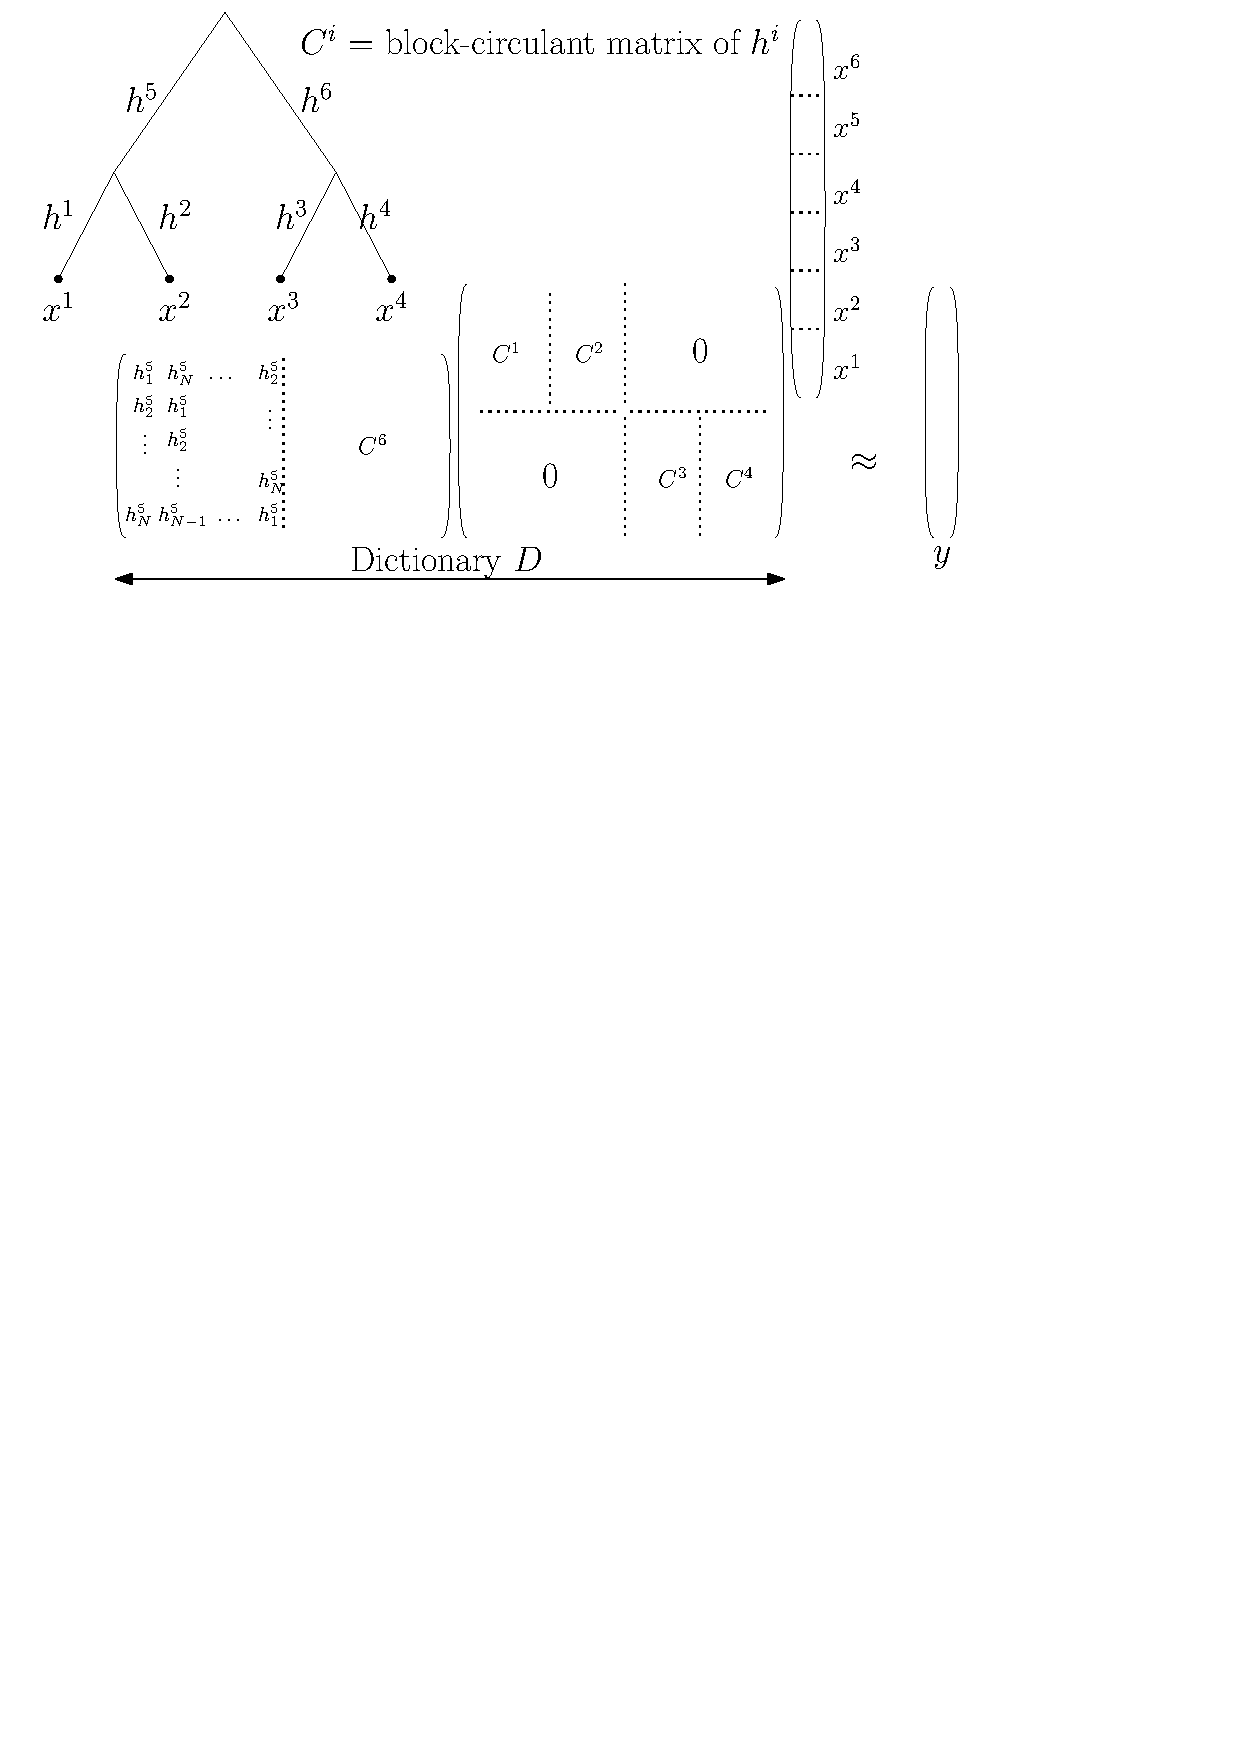
\includegraphics[width=0.8\textwidth]{figures/block-circular-matrix.pdf}
	\caption{This figure shows how to go from the tree defined by its kernels $(\h^e)_{e \in \E}$ to a matrix $\D$} \label{fig_block_circular}
\end{figure}

\section{Why is sparse coding used for denoising?}

The figure \ref{sparse_reduce_noise} shows a noisy signal $\y$ living in a high-dimensional $N$ and defined by
$$\y=\hat{\y} + b$$
with $b$ following a centered Gaussian distribution $\mathcal{N}(0,\sigma^2I)$ and $\hat{\y}$ the noise-less signal. We see that the distance $||b||$ is always lower than the projected distance.

This is because the deviation in the $N$ dimensional space can be written as
\begin{align*}
\sigma^2(b) =& \mathbb{E}\left[\lVert b-\mathbb{E}(b) \rVert^2 \right]\\
=& \mathbb{E}\left(\lVert b \rVert^2 \right)\\
=& ... \\ % TODO finish useless proof
=& \frac{1}{N}\lVert b \rVert^2
\end{align*}
which gives 
$$ \lVert b \rVert = \sigma\sqrt{N} $$
When projected to the $K$ dimensional space, the noise deviation becomes
$$\lVert b \rVert = \sigma\sqrt{K} $$
which is much better than the previous distance, provided that $K<<N$. 

\begin{figure}[!ht]\centering
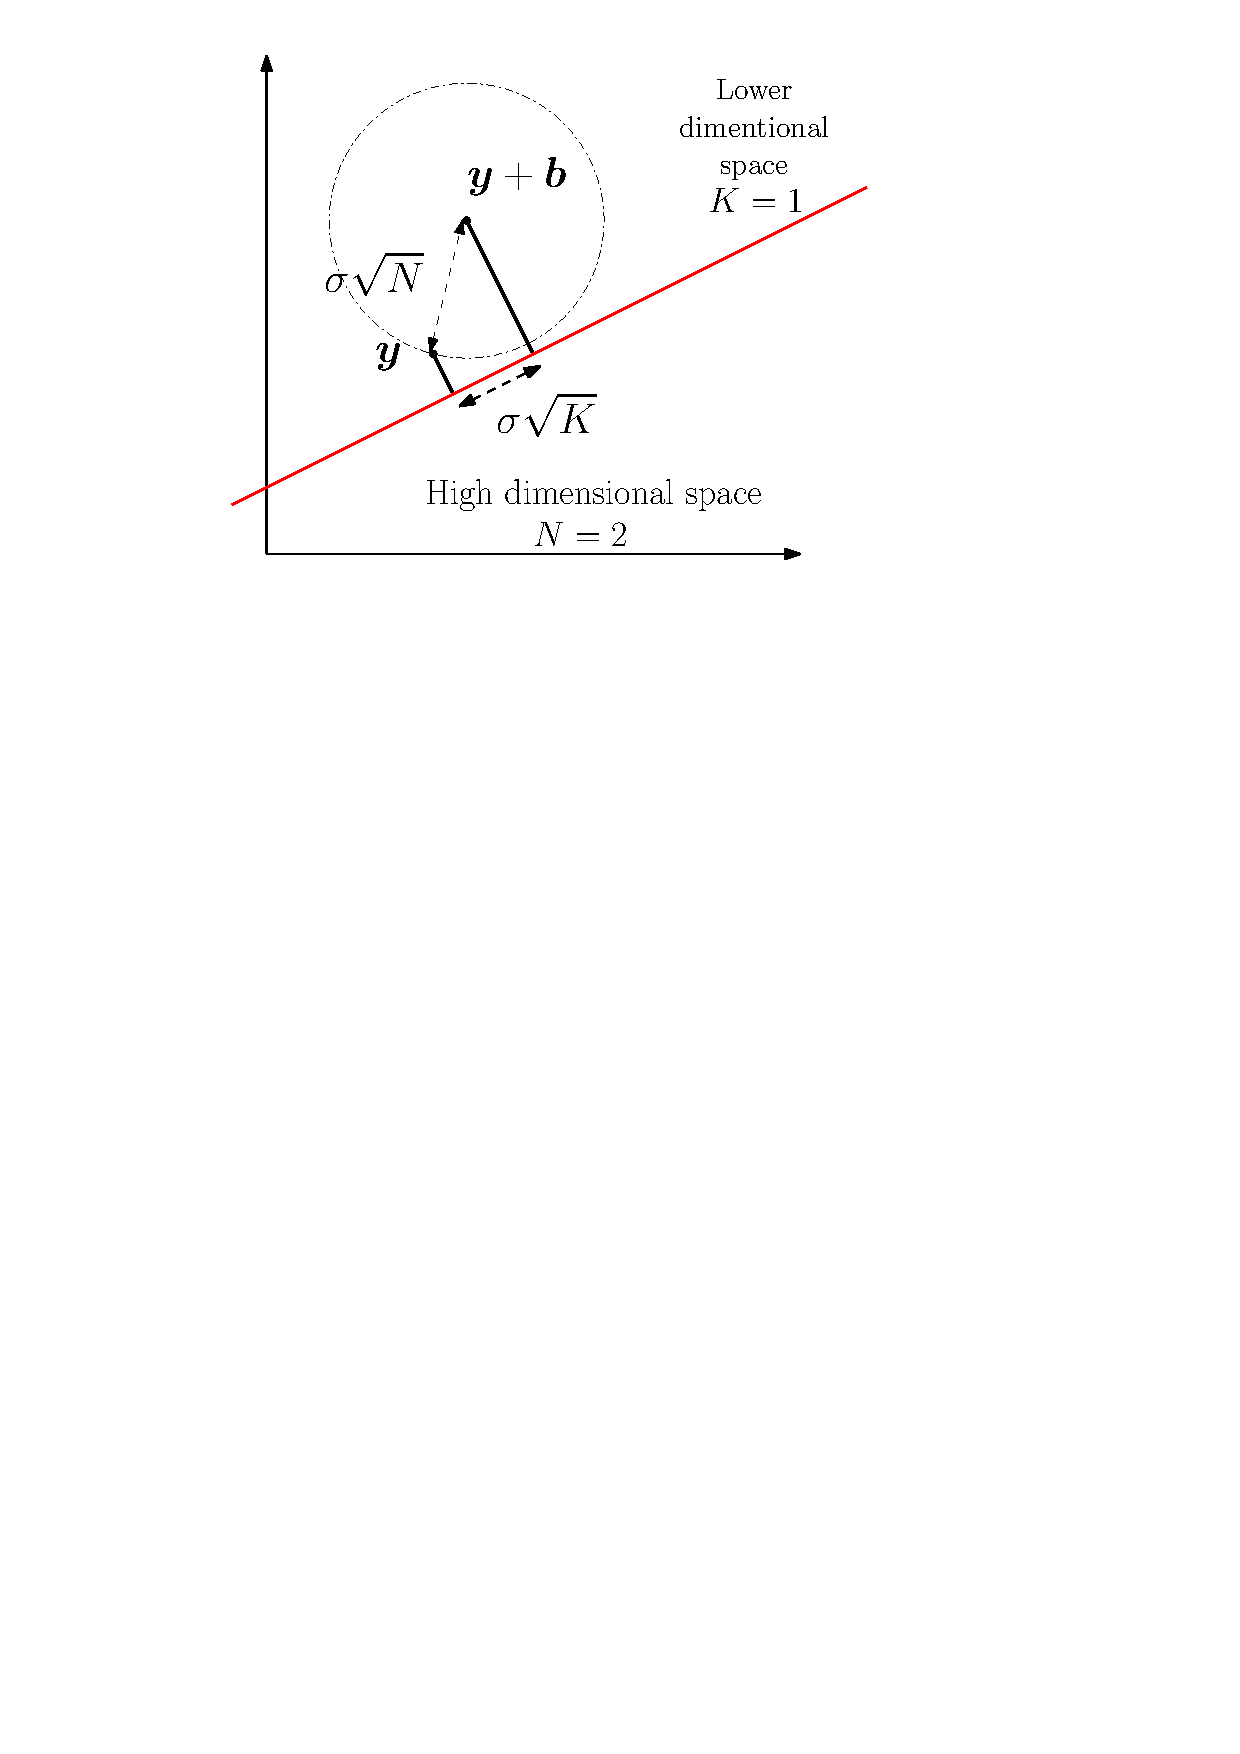
\includegraphics[width=0.4\textwidth]{figures/sparse-reduce-noise.pdf}
\caption{When projected onto a lower dimensional space, the standard derivation of the additive Gaussian noise $b \sim \mathcal{N}(0,\sigma^2)$ will be greatly reduced if $K<<N$. The sparser the representation the better the denoising. \label{sparse_reduce_noise}}
\end{figure}

\section{Why $FT(\widetilde{A}) = FT(A)^*$}
\begin{align*}
(\widehat{\widetilde{A}})_{m,n} =& \sum_{k=1}^M \sum_{l=1}^N \widehat{A}_{k,l} e^{-2i\pi (k\frac{m}{M}+l \frac{n}{N})}\\
=& \sum_{k=1}^M \sum_{l=1}^N A_{-k,-l} e^{-2i\pi (k\frac{m}{M}+l \frac{n}{N})}\\
\shortintertext{By changing variables $k'=-k$ and $l'=-l$, we get:}
=& \sum_{k'=-M}^{-1} \sum_{l'=-N}^{-1} A_{k',l'} e^{2i\pi (k'\frac{m}{M}+l' \frac{n}{N})}
\shortintertext{And thanks to the $(M,N)$ periodicity of $A$, which means that $A_{i,j}=A_{i+kM,j+lN}$, $\forall (k,l) \in \mathbb{N}^2$, letting us with:}
=& \sum_{k'=-M}^{-1} \sum_{l'=-N}^{-1} A_{k'+M,l'+N} e^{2i\pi (k'\frac{m}{M}+l' \frac{n}{N})}\\
\shortintertext{With a second change of variables $k''=k'+M$ and $l''=l'+N$:}
=& \sum_{k''=-M+M}^{-1+M} \sum_{l''=-N+N}^{-1+N} A_{k'',l''} e^{2i\pi (k'\frac{m}{M}+l' \frac{n}{N})}\\
=& \sum_{k'=1}^{M} \sum_{l'=1}^{N} A_{k',l'} e^{2i\pi (k'\frac{m}{M}+l' \frac{n}{N})}
\end{align*}
% TODO Proof not finished; this proof might be useless/overkill in my thesis...


\printbibliography

\end{document}



